%% Experimental validation -- fluidization
\frame{
\begin{tikzpicture}[remember picture,overlay]
\fill[blue1]
(current page.north west) rectangle ([xshift=0.57\textwidth,yshift=0.28\textheight]current page.west|-{pic cs:end});
\end{tikzpicture}

\begin{textblock}{0.53}(0.02,0.03)
	\textcolor{white}{
	\Large Experimental validation of X-DFA: \\
	A suspension of sedimenting particles}
\end{textblock}

\begin{textblock}{0.57}(0.02,0.18)
\centering
\only<1>{
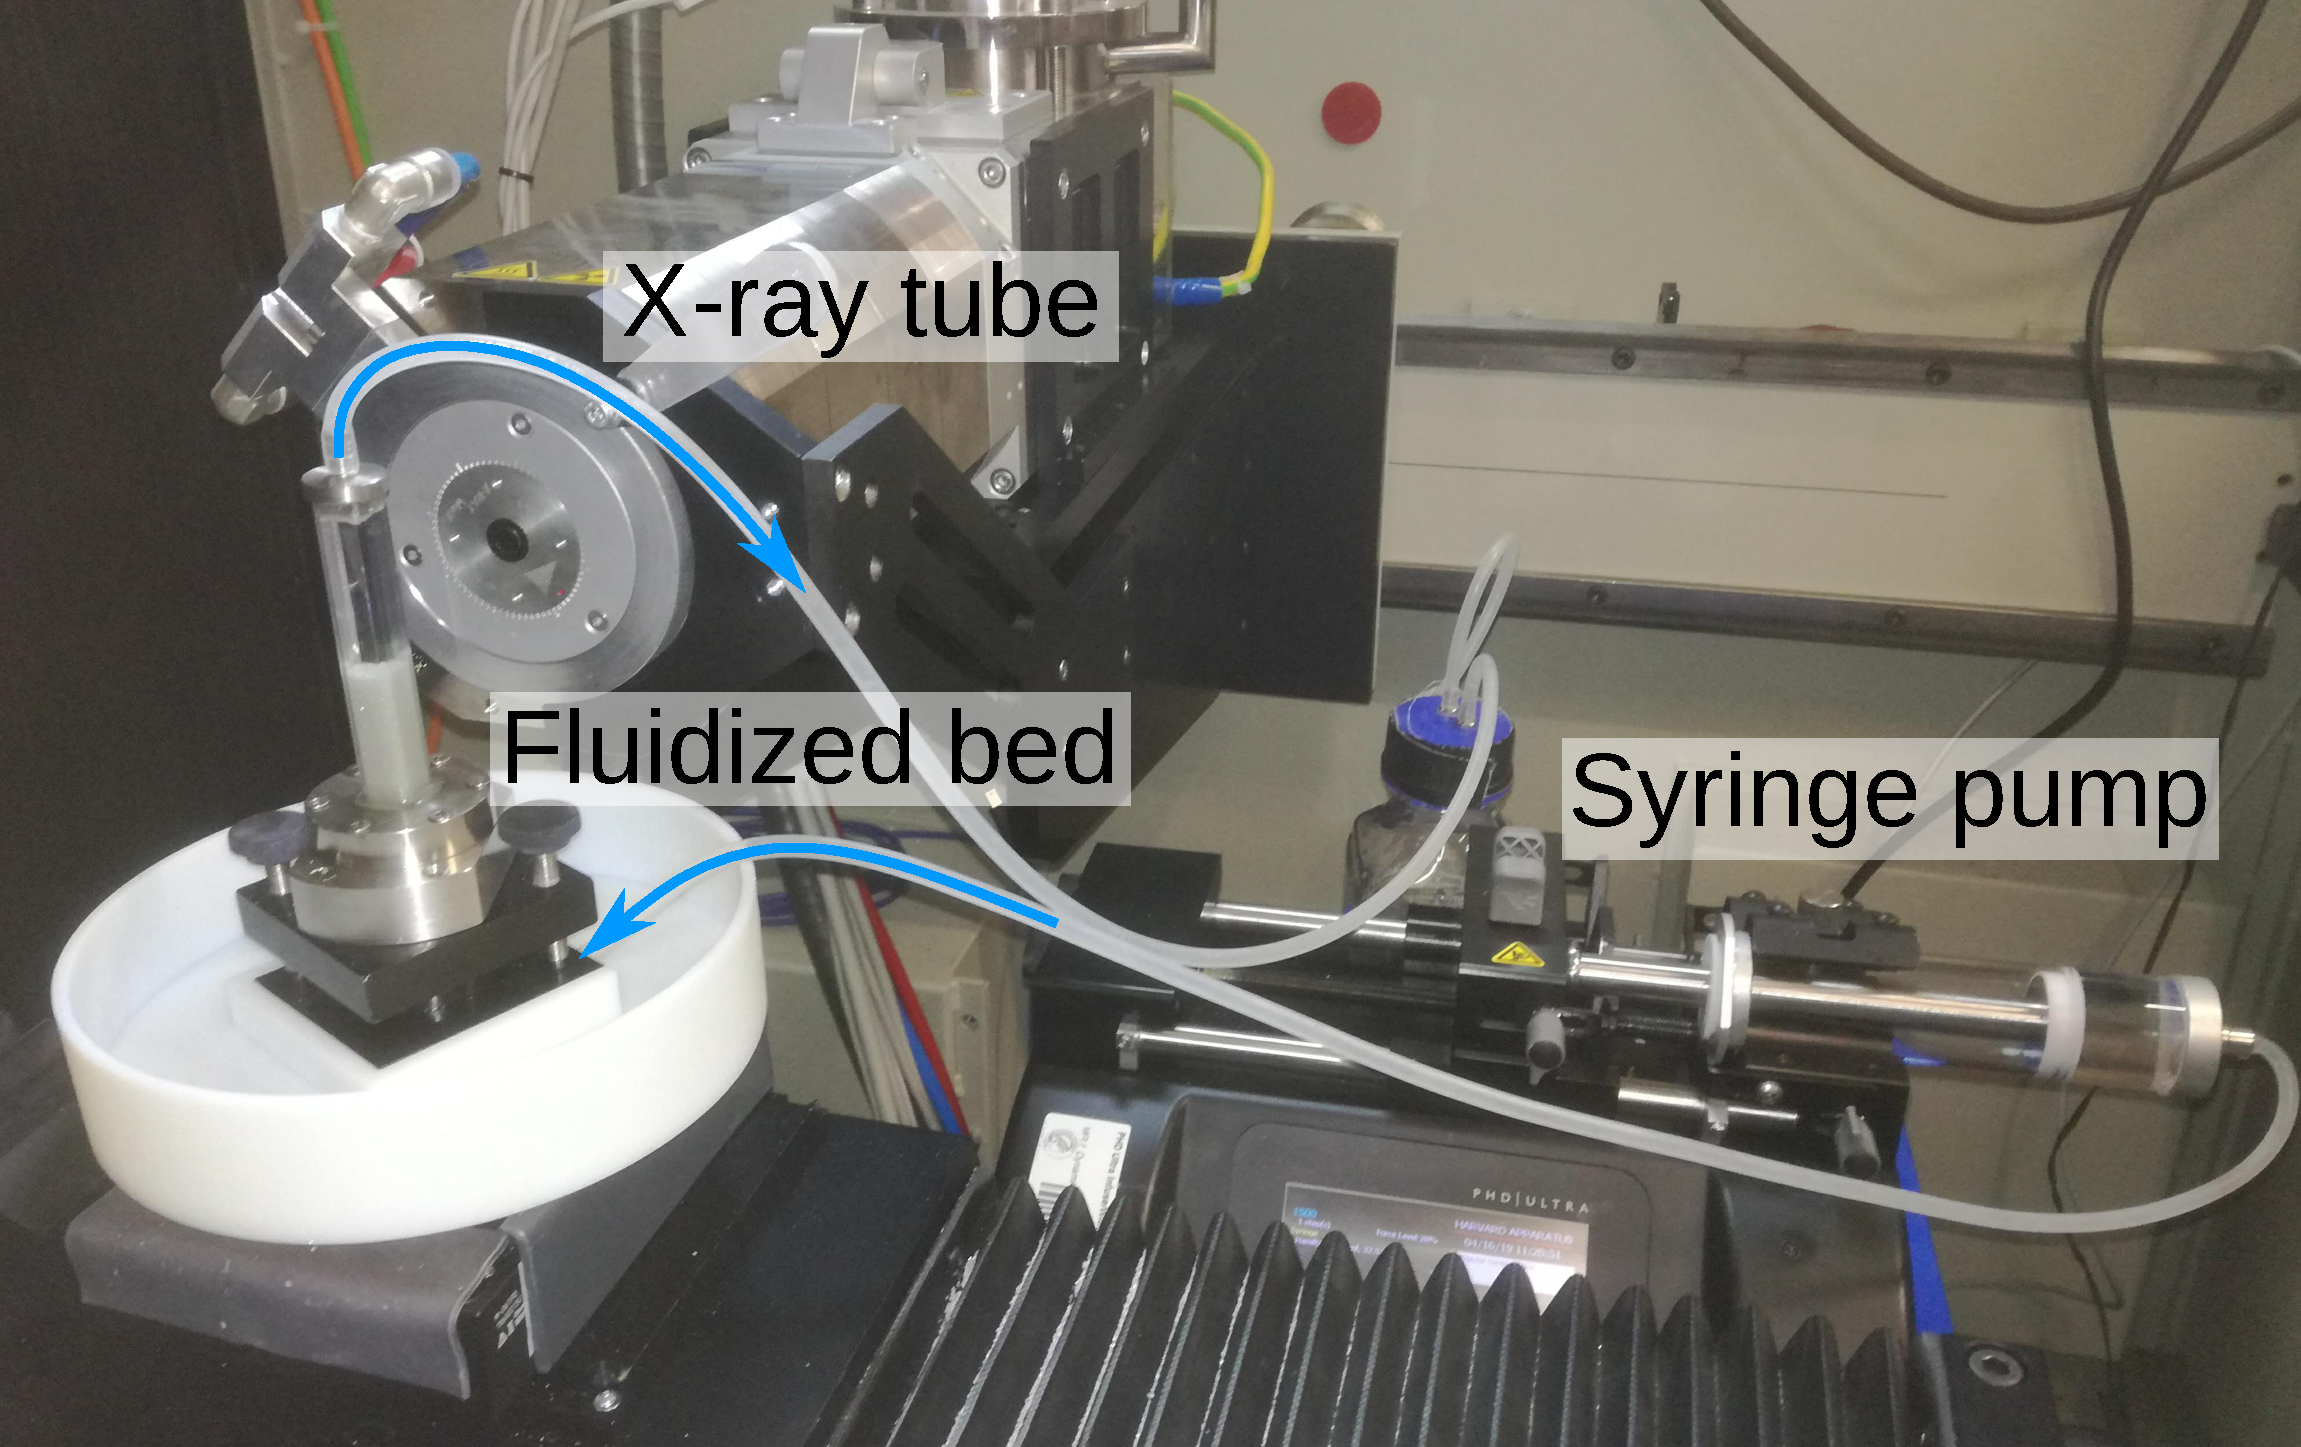
\includegraphics[width=\textwidth]{Sources/sedimenting_bed/Photo_fluidized_bed.pdf}
}
\visible<2->{
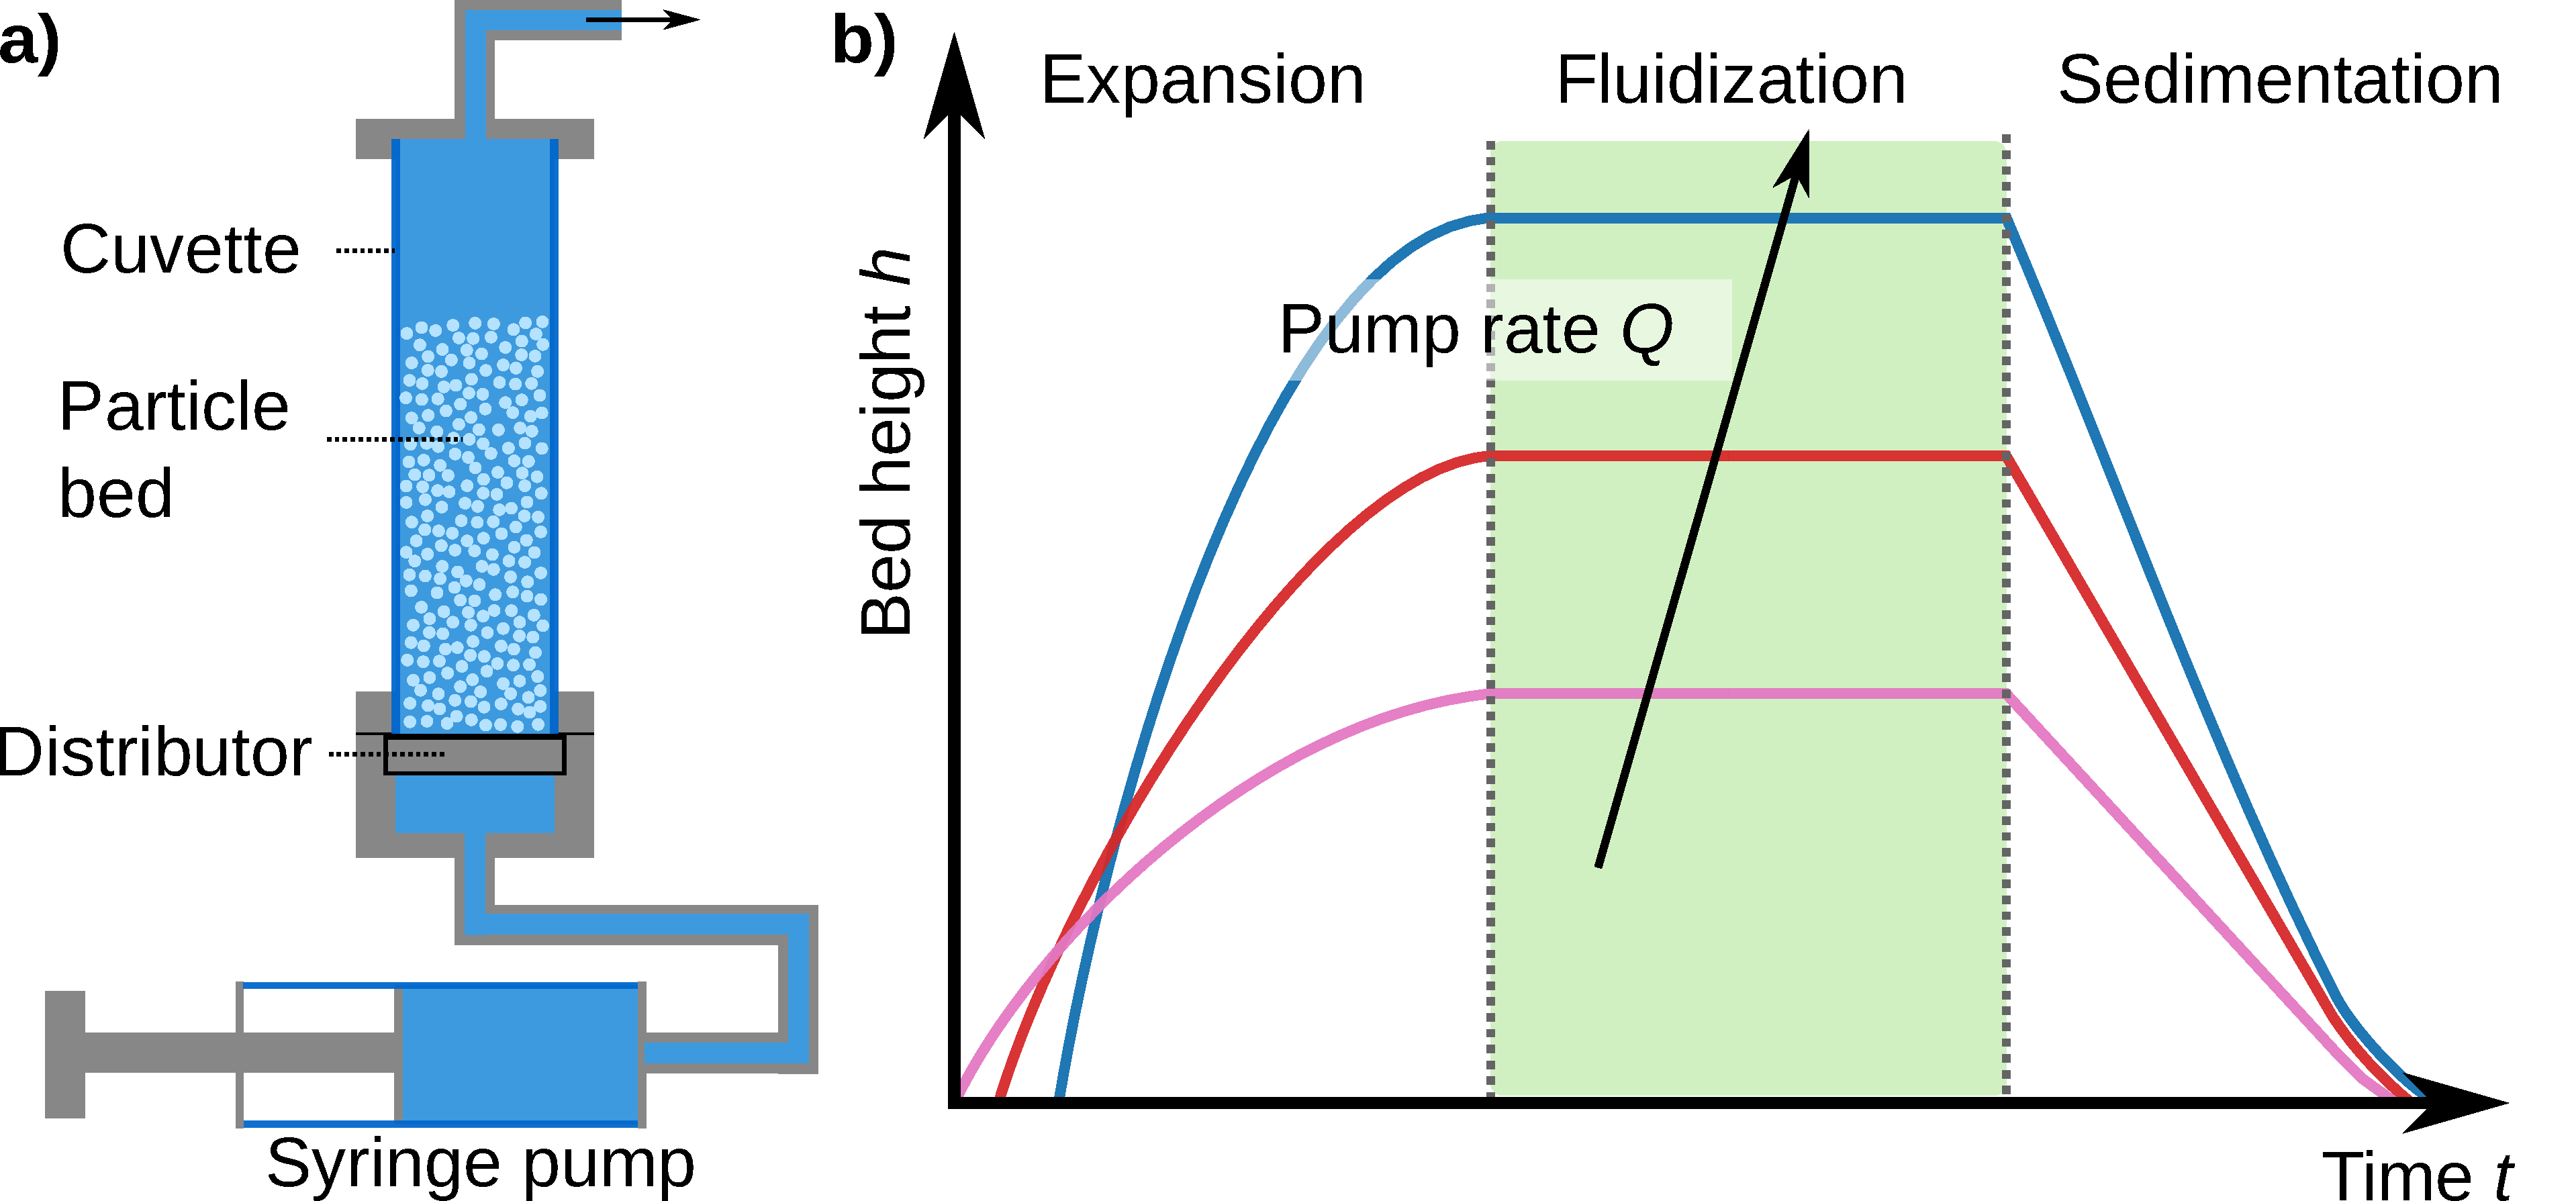
\includegraphics[width=\textwidth]{Sources/sedimenting_bed/setup-fluidized_bed_fluidized.pdf}}
\end{textblock}	

\begin{textblock}{0.32}(0.64,0.18)	
	\visible<2->{
	\centering
	X-ray radiography\\[0.1cm]
	\fbox{\parbox{\textwidth}{
	\movie[width =\textwidth, poster, loop]
	{\includegraphics[width=\textwidth]{Sources/sedimenting_bed/Radiogram_plane0.png}}
	{videos/full_fluidization.avi}}}}
\end{textblock}

\begin{textblock}{0.15}(0.22,0.75)
	\only<3>{
	\textcolor{red}{No reliable reference velocity!}
	}
\end{textblock}

\begin{textblock}{0.17}(0.34,0.64)
	\only<3>{
	\fbox{\parbox{\textwidth}{
			\movie[width =\textwidth, poster, loop]
			{
\includegraphics[width=\textwidth]{Sources/X-DFA/cropped_80kV_340uA_38ms_0000.png}}
			{videos/fluidized_3500mul_per_min.avi}}}
		}
\end{textblock}
}


%%%%%%%%% sedimentation
\begin{frame}
\begin{tikzpicture}[remember picture,overlay]
\fill[blue1]
(current page.north west) rectangle ([xshift=0.57\textwidth,yshift=0.28\textheight]current page.west|-{pic cs:end});
\end{tikzpicture}

\begin{textblock}{0.53}(0.02,0.03)
	\textcolor{white}{
		\Large Experimental validation of X-DFA: \\
		A suspension of sedimenting particles}
\end{textblock}

	
\begin{textblock}{0.57}(0.02,0.18)
	\centering
	\visible<1->{
	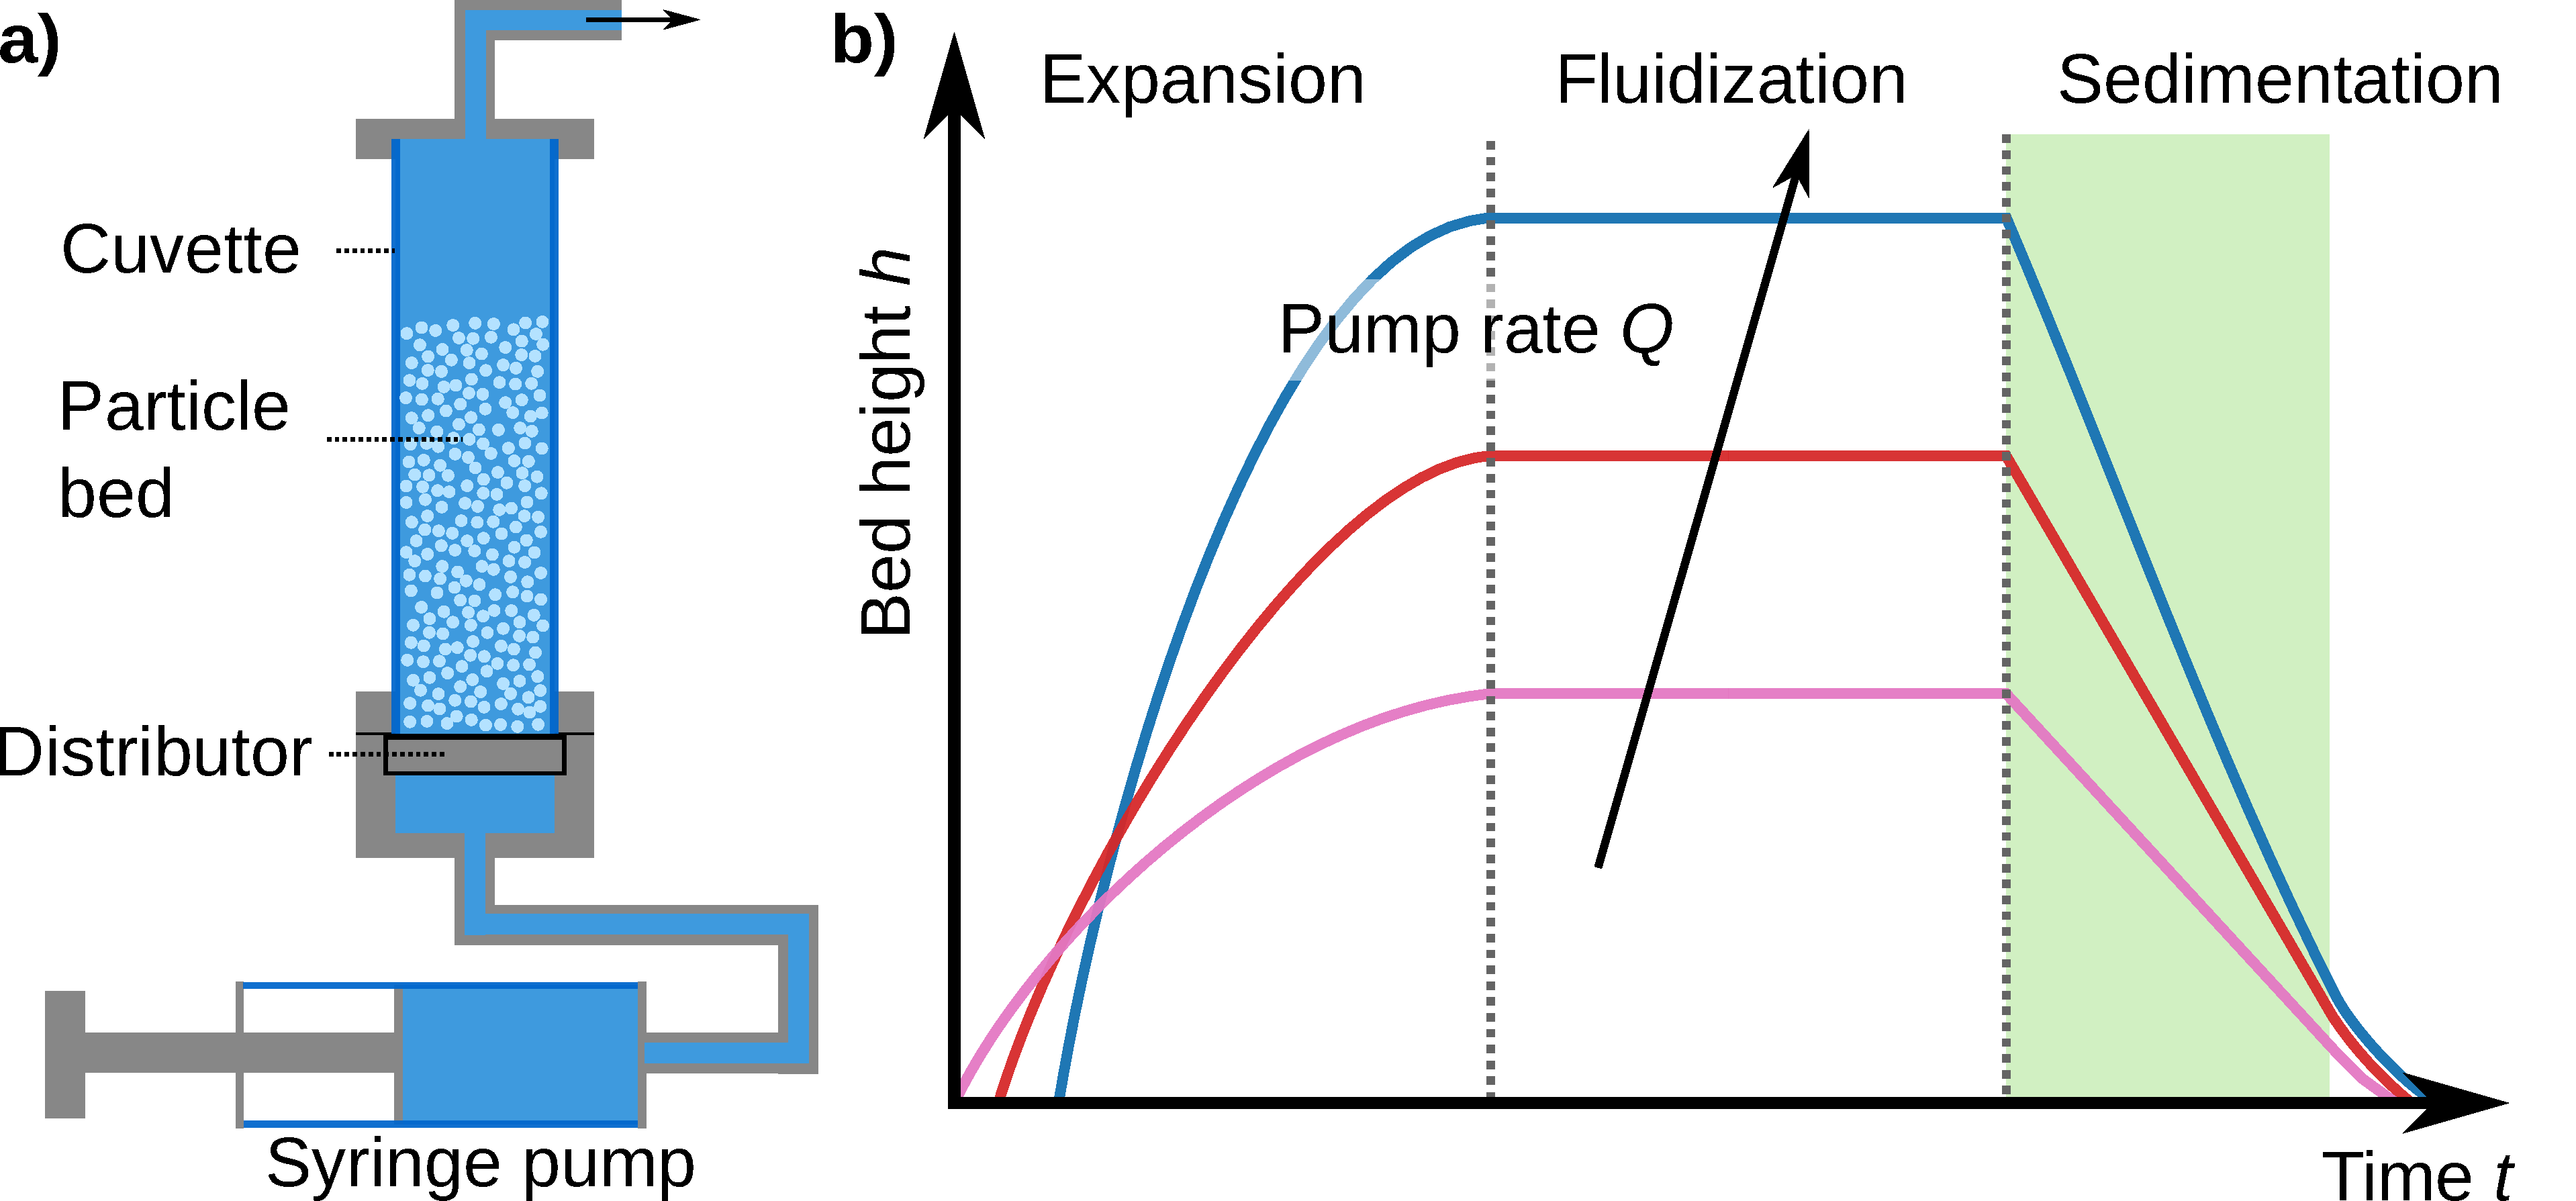
\includegraphics[width=\textwidth]{Sources/sedimenting_bed/setup-fluidized_bed.pdf}}
\end{textblock}	

\begin{textblock}{0.32}(0.64,0.05)
	\centering
	X-ray radiography\\[0.1cm]
	\only<1>{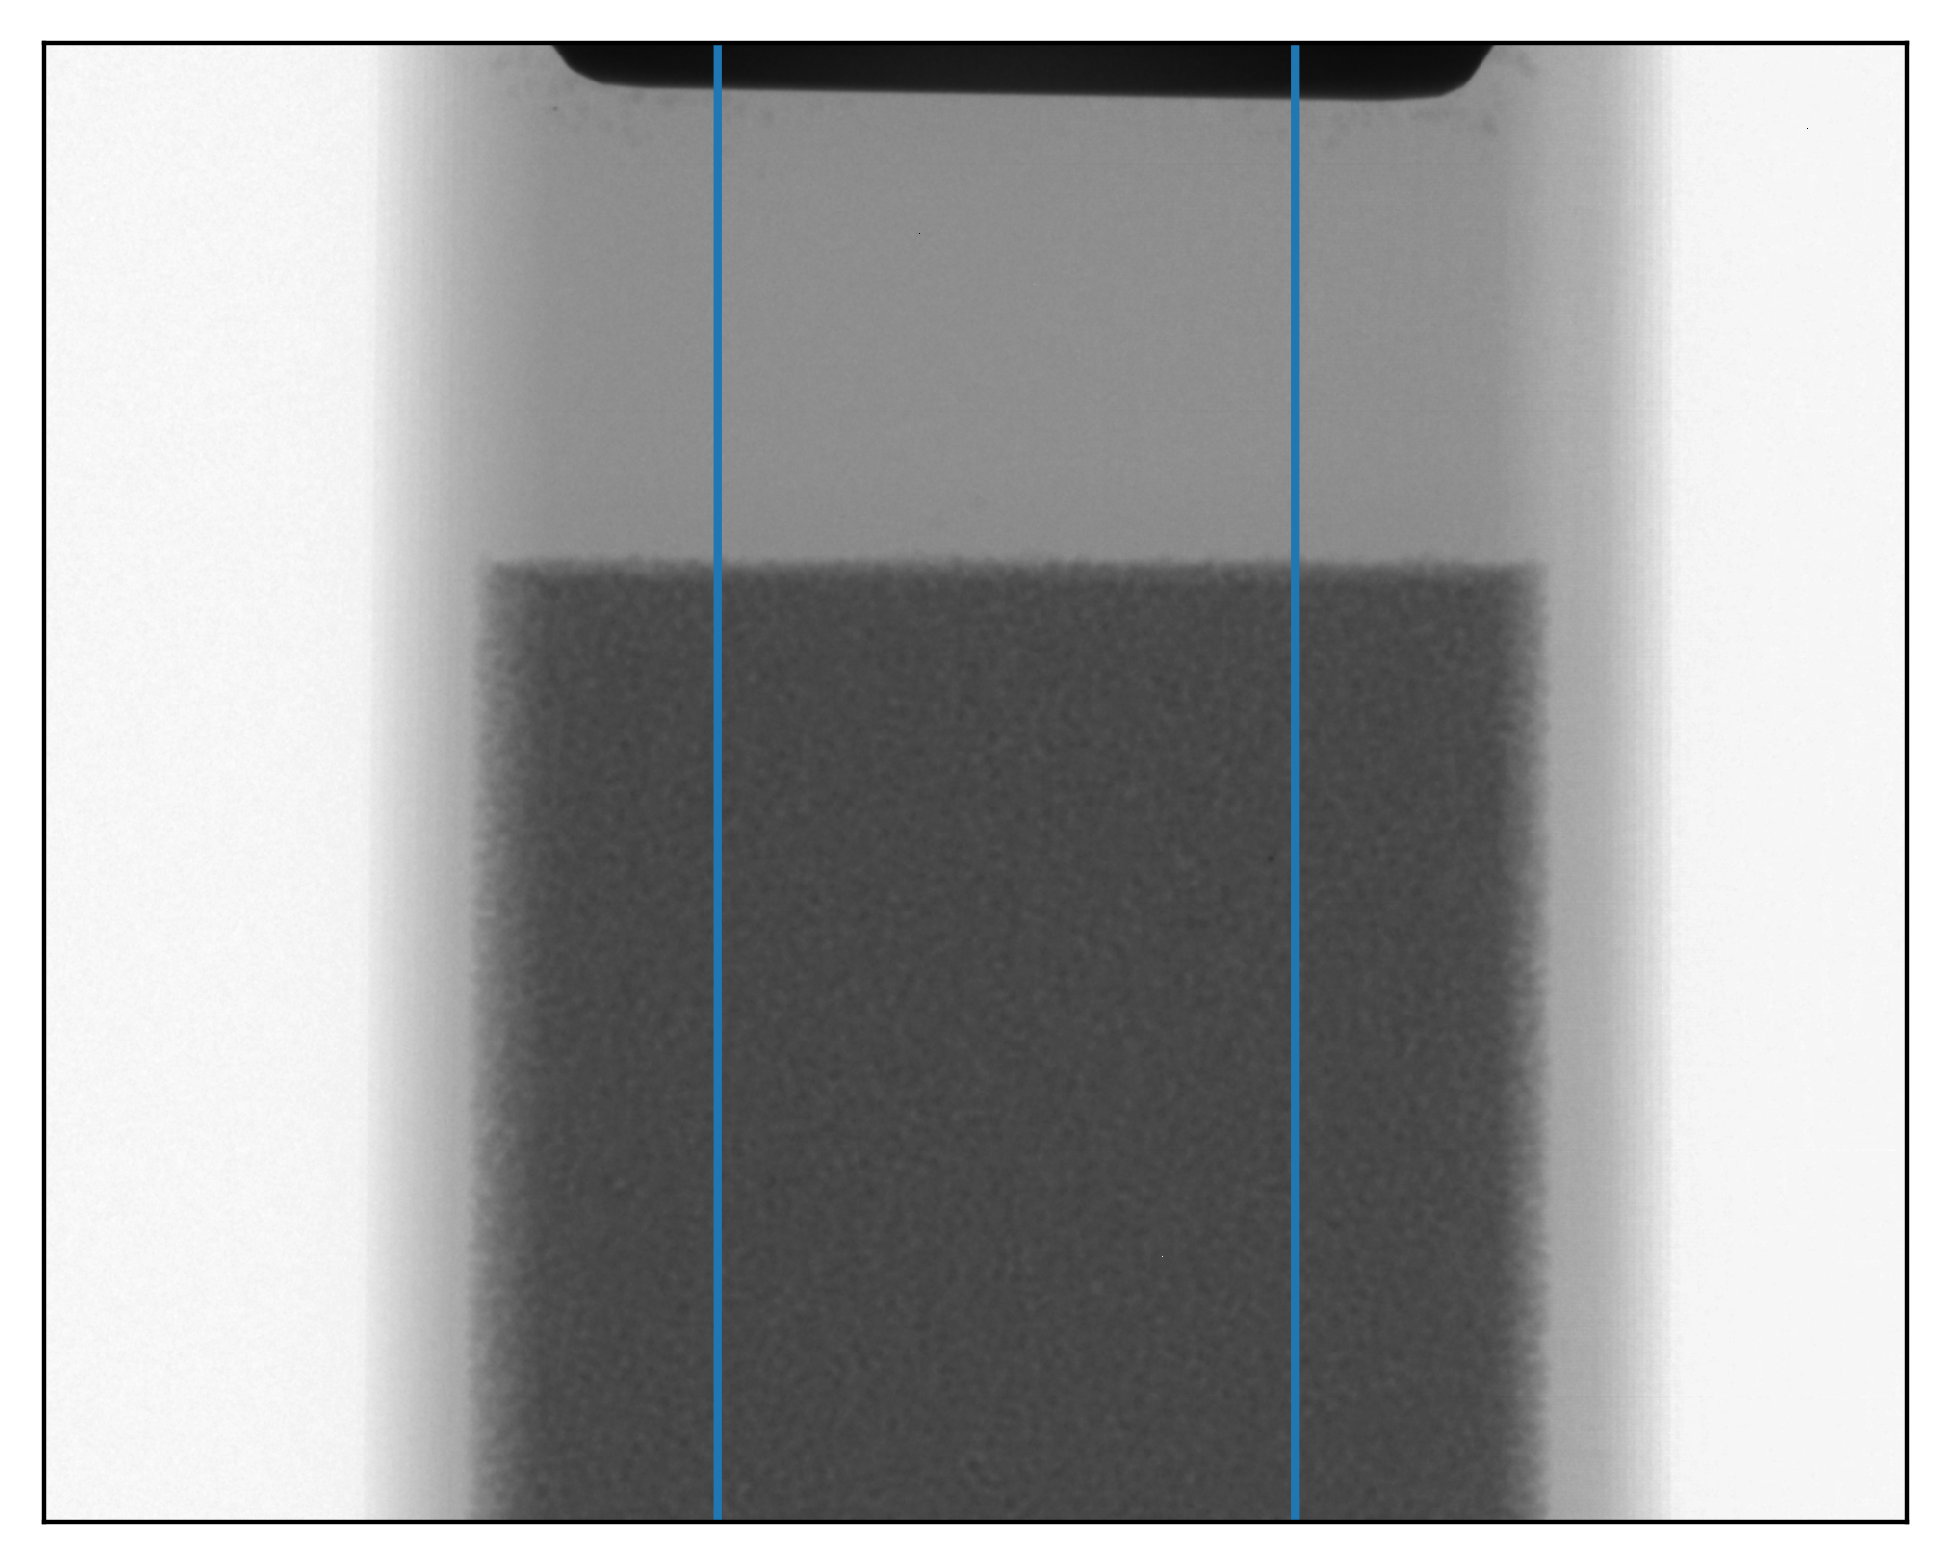
\includegraphics[width=\textwidth]{Sources/sedimenting_bed/ROI_marked_img_nr1.png}}
	\visible<2->{
	\fbox{\parbox{0.62\textwidth}{
	\movie[width = 0.62\textwidth, poster]
	{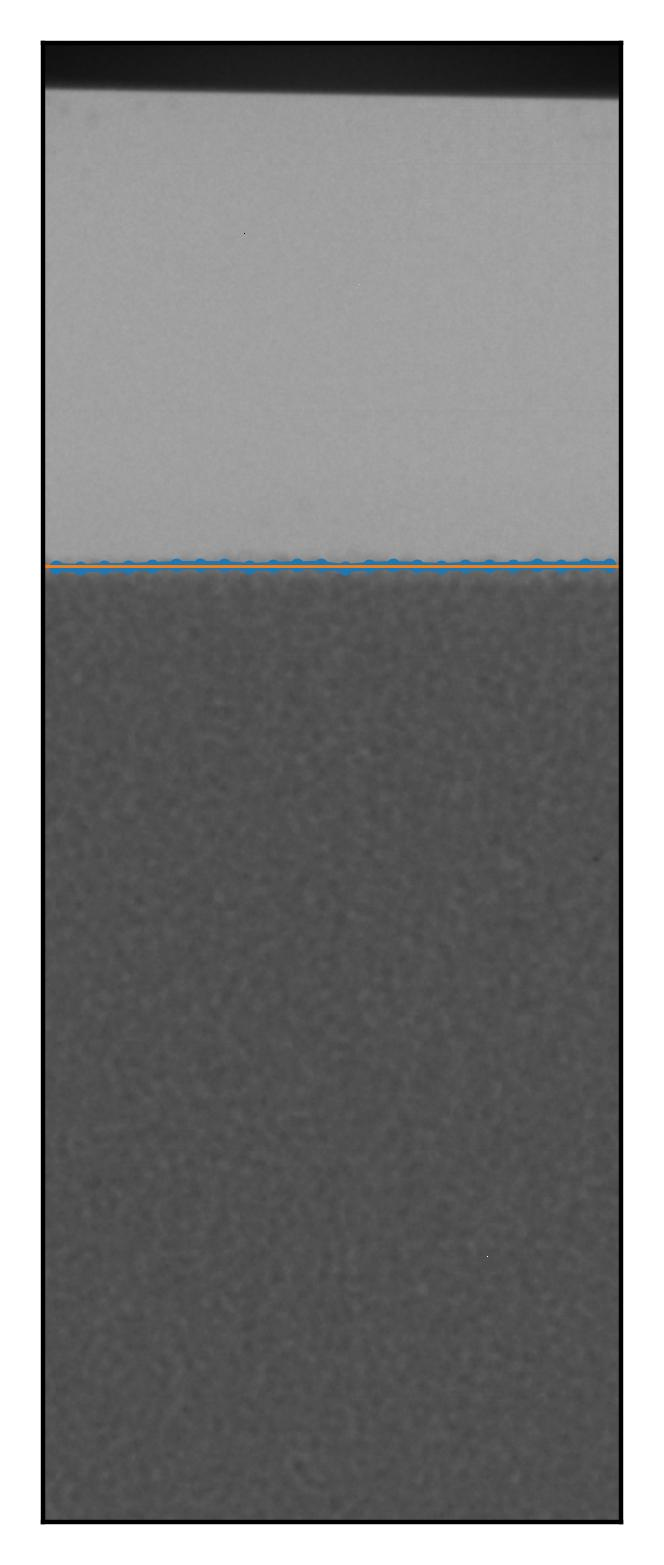
\includegraphics[width=.62\textwidth]{Sources/sedimenting_bed/tracked_edge0.png}}
	{videos/tracked_edge.avi}}}}
\end{textblock}

\begin{textblock}{0.17}(0.28,0.64)
	\visible<2->{
		\fbox{\parbox{\textwidth}{
		\movie[width =\textwidth, poster, loop]
		{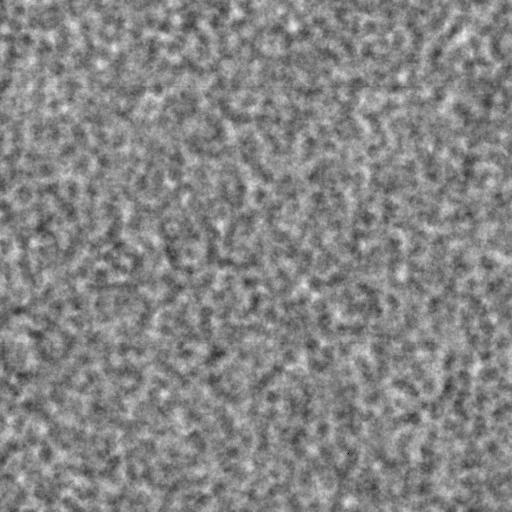
\includegraphics[width=\textwidth]{Sources/sedimenting_bed/sedimentationROI.png}}
		{videos/02_750ul_per_min_original.avi}}}
	}
\end{textblock}

\begin{textblock}{0.25}(0.45,0.75)
\visible<2->{
\centering
\textcolor{blue1}{
Comparison of \\
$\langle v \rangle_\text{xdfa}$ and $\langle v \rangle_\text{front}$}
}
\end{textblock}
\end{frame}






%% ISF X-DFA experiment
\frame{
\begin{tikzpicture}[remember picture,overlay]
\fill[blue1]
(current page.north west) rectangle ([xshift=0.4\paperwidth,yshift=0.28\textheight]current page.west|-{pic cs:end});
\end{tikzpicture}

\begin{textblock}{0.8}(0.02,0.03)
	\textcolor{white}{
		\Large X-DFA for a suspension of \\
		sedimenting particles$^{(1)}$}
\end{textblock}	

\begin{textblock}{0.45}(0.5,0.05)
\fbox{\parbox{\textwidth}{
\begin{minipage}[c]{0.25\textwidth}
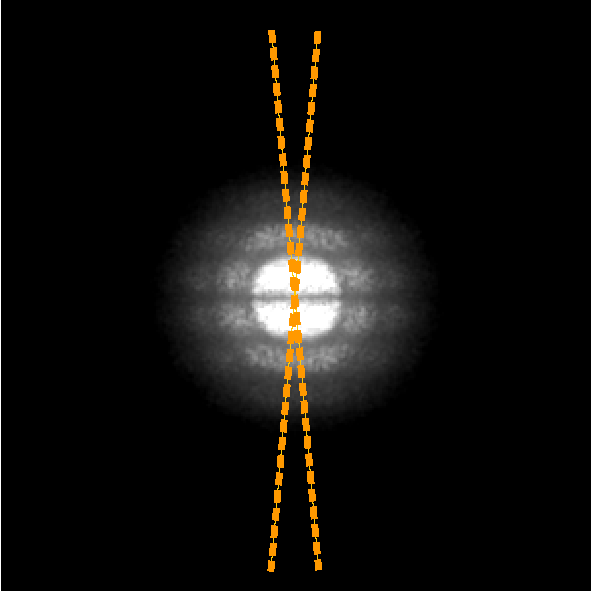
\includegraphics[width=\textwidth]
{Sources/sedimenting_bed/structure_func_angle.pdf}
\end{minipage}
\hfill
\begin{minipage}[c]{0.7\textwidth}
Image structure function:\\
$D(\mathbf{q},\tau) = 
\langle | \mathcal{F} [\Delta I (\mathbf{r}, t, \tau)] |^2\rangle_t$
\end{minipage}
}}
\end{textblock}

\begin{textblock}{0.45}(0.02,0.38)	
	\centering
	\visible<2->{
		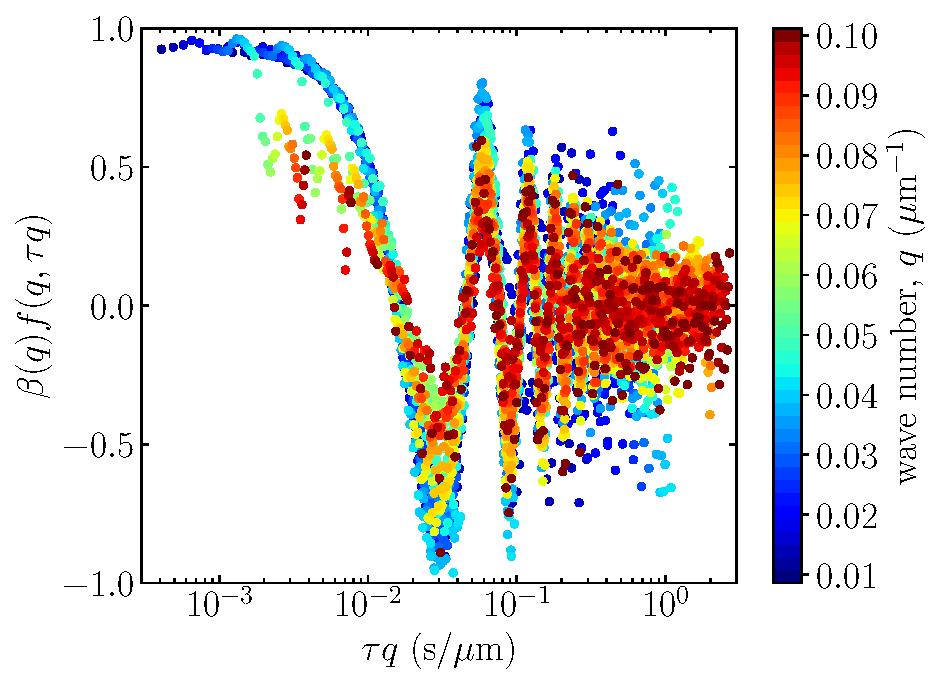
\includegraphics[height=0.57\textheight]
		{Sources/sedimenting_bed/fqt_tq.pdf}}
\end{textblock}

\begin{textblock}{0.4}(0.02,0.18)
	\only<2>{
	Intermediate scattering function$^{(2)}$:
	\begin{align}
	f(q,\tau) = 
	\cos(q \langle v_\text{s} \rangle \tau)
	\exp\left(- \frac{1}{2} q^2 \delta v^2 \tau^2 \right)
	\nonumber
	\end{align}
	}
	\visible<3->{
	Intermediate scattering function$^{(2)}$:
	\begin{align}
	f(q,\tau) = 
	\cos(q \textcolor{orange}{\langle v_\text{s} \rangle} \tau)
	\exp\left(- \frac{1}{2} q^2 \textcolor{darkgreen}{\delta v^2} \tau^2 \right)
	\nonumber
	\end{align}
	}
\end{textblock}


\begin{textblock}{0.4}(0.55,0.25)
\visible<3->{
\begin{align}
\textcolor{orange}{
	\langle v_\text{s} \rangle = q\ \tau_\nu} &&
\textcolor{darkgreen}{
	\delta v = q\ \tau_{\delta \nu}}
\nonumber
\end{align}
}
\end{textblock}


\begin{textblock}{0.45}(0.5,0.4)	
	\centering
	\visible<4->{
	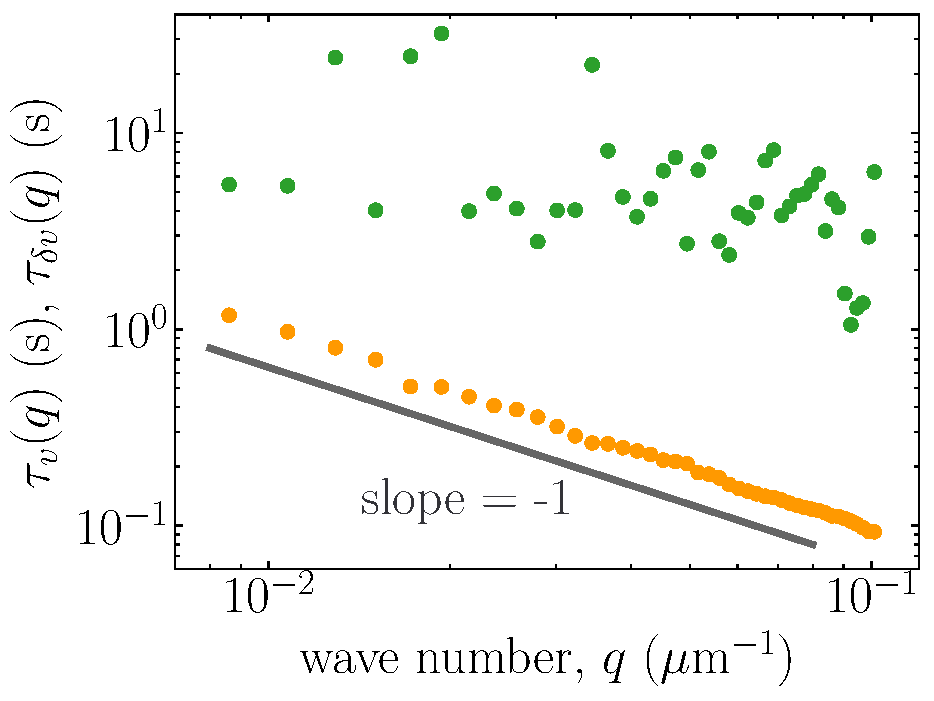
\includegraphics[height=0.55\textheight]
	{Sources/sedimenting_bed/tau_vs_q.pdf}}
\end{textblock}

\begin{textblock}{0.9}(0.02,0.95)
	{\scriptsize
	${(1)}$ In collaboration with Manuel Escobedo, University of Düsseldorf}
\end{textblock}

\begin{textblock}{0.9}(0.6,0.95)
	\visible<2->{
	{\scriptsize
	${(2)}$ Kohyama \textit{et al.} (2008)}}
\end{textblock}
}





%%%%%%%%%%% Front tracking vs X-DFA %%%%%%%%%%%%%%%%%%%%%
\frame{
\begin{tikzpicture}[remember picture,overlay]
\fill[blue1]
(current page.north west) rectangle ([xshift=0.38\paperwidth,yshift=0.33\paperheight]current page.west|-{pic cs:end});
\end{tikzpicture}

\begin{textblock}{0.8}(0.02,0.03)
	\textcolor{white}{
		\Large Front tracking vs.\ X-DFA}
\end{textblock}

\begin{textblock}{0.45}(0.02,0.1)	
\centering
\only<1>{
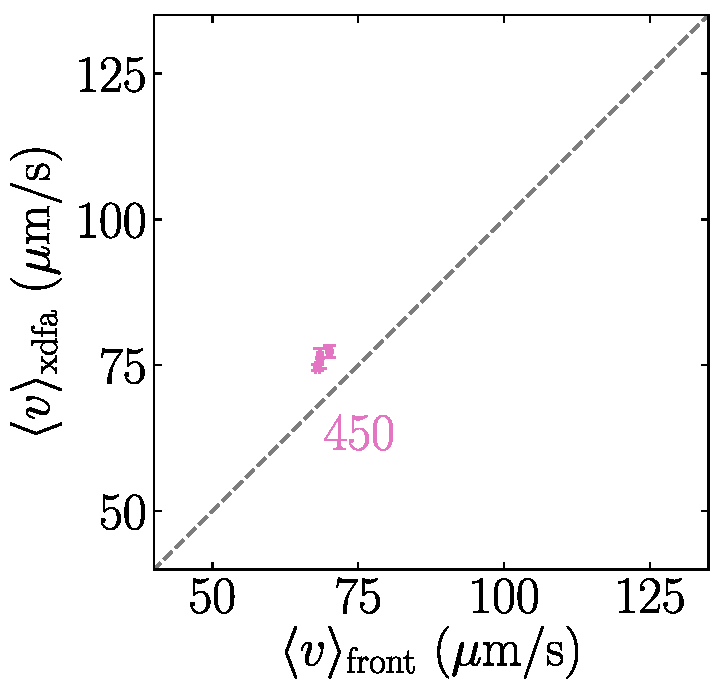
\includegraphics[width=\textwidth]
{Sources/sedimenting_bed/velocity_comp_1.pdf}}
\only<2>{
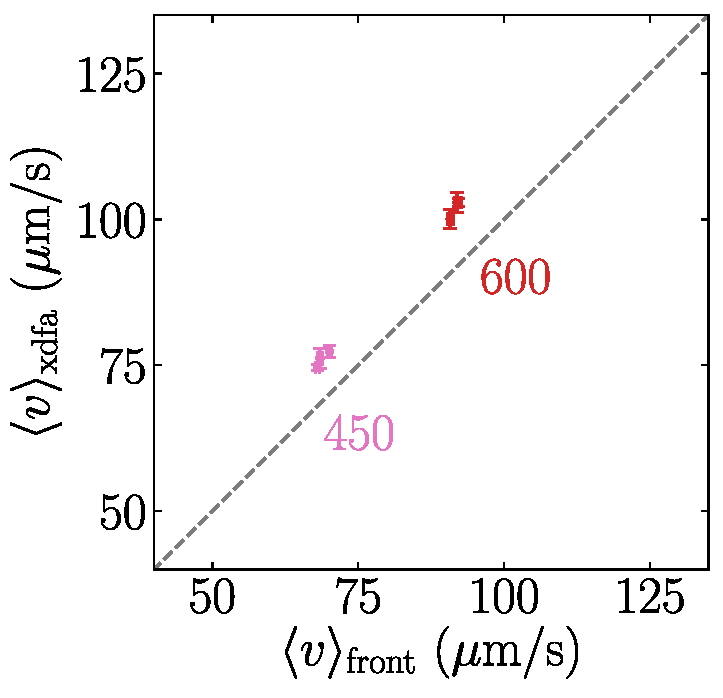
\includegraphics[width=\textwidth]
{Sources/sedimenting_bed/velocity_comp_2.pdf}}
\only<3>{
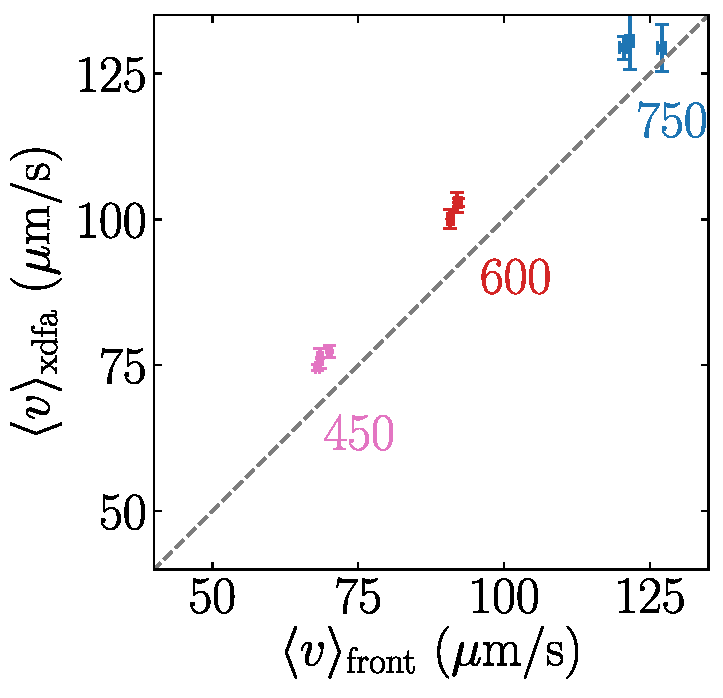
\includegraphics[width=\textwidth]
{Sources/sedimenting_bed/velocity_comp_3.pdf}}
\visible<4->{
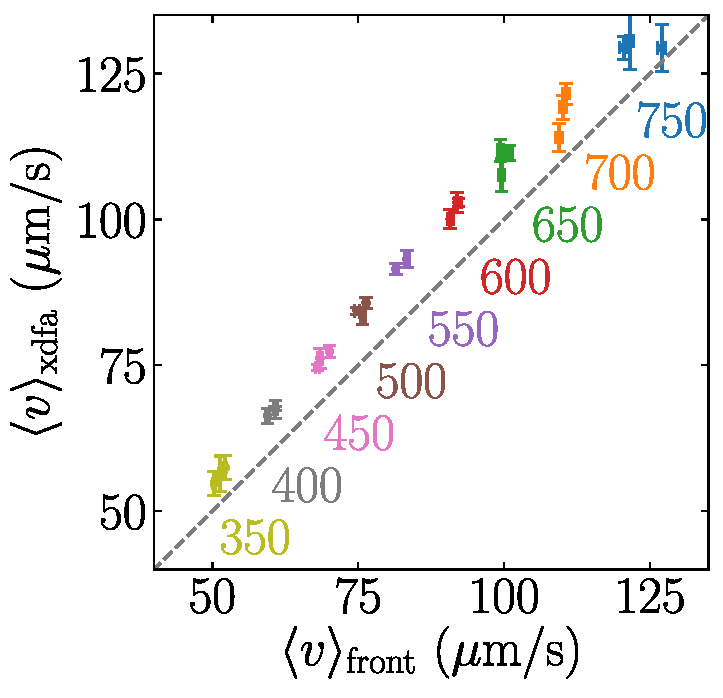
\includegraphics[width=\textwidth]
{Sources/sedimenting_bed/velocity_comp_final.pdf}}
\end{textblock}

\begin{textblock}{0.5}(0.55,0.05)
\only<1>{
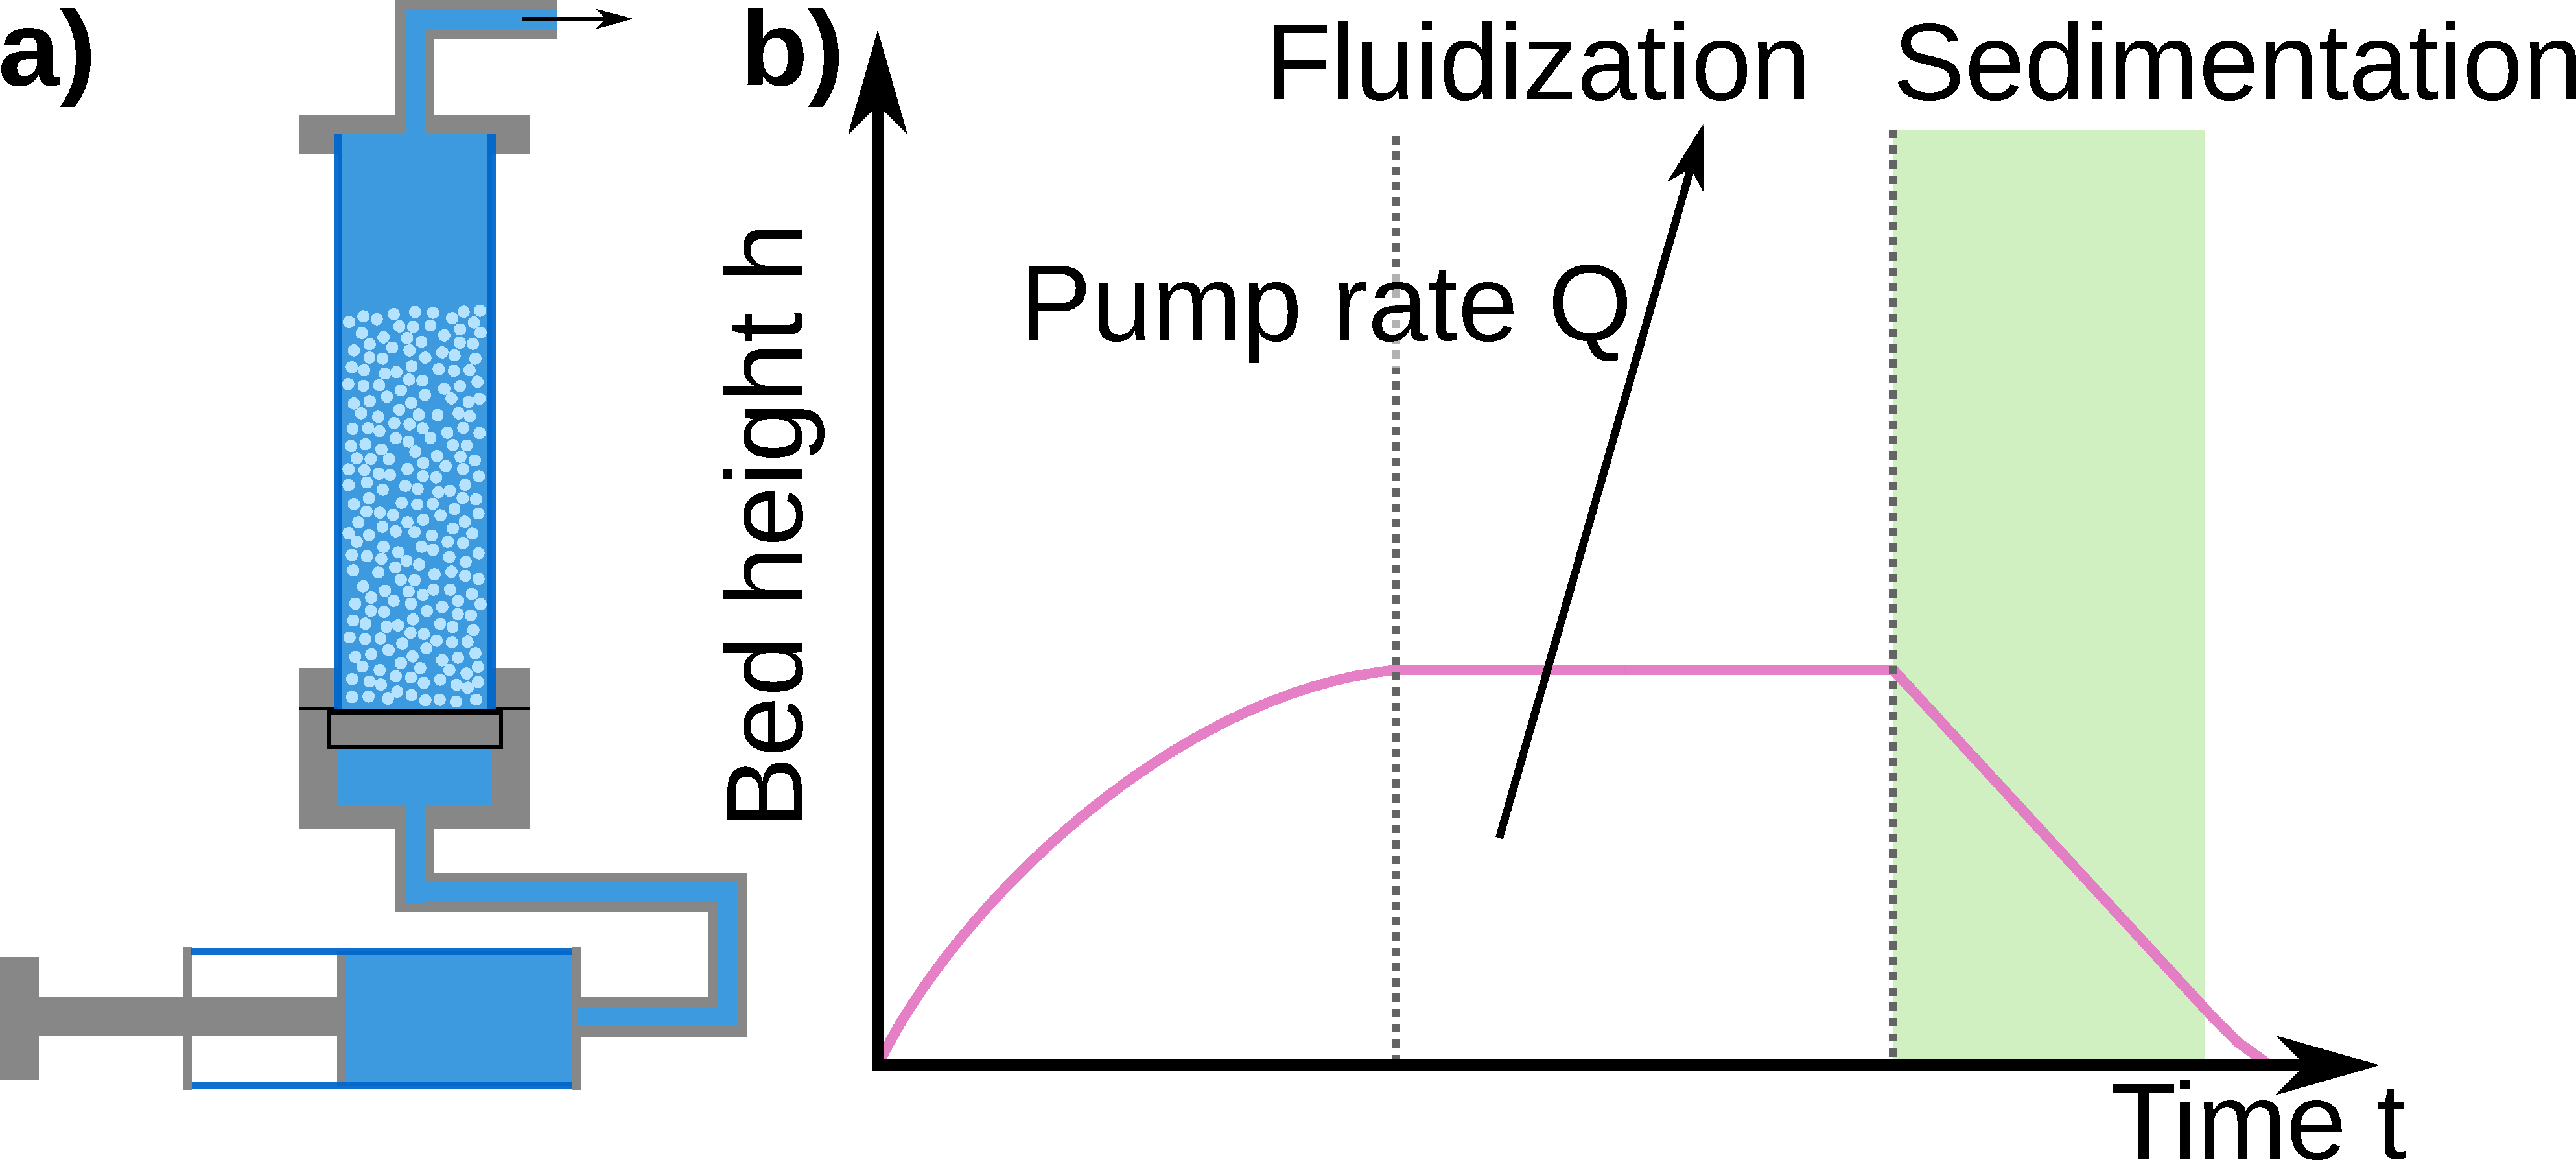
\includegraphics[width=0.8\textwidth]
{Sources/sedimenting_bed/setup-fluidized_bed_animation_1.pdf}}
\only<2>{
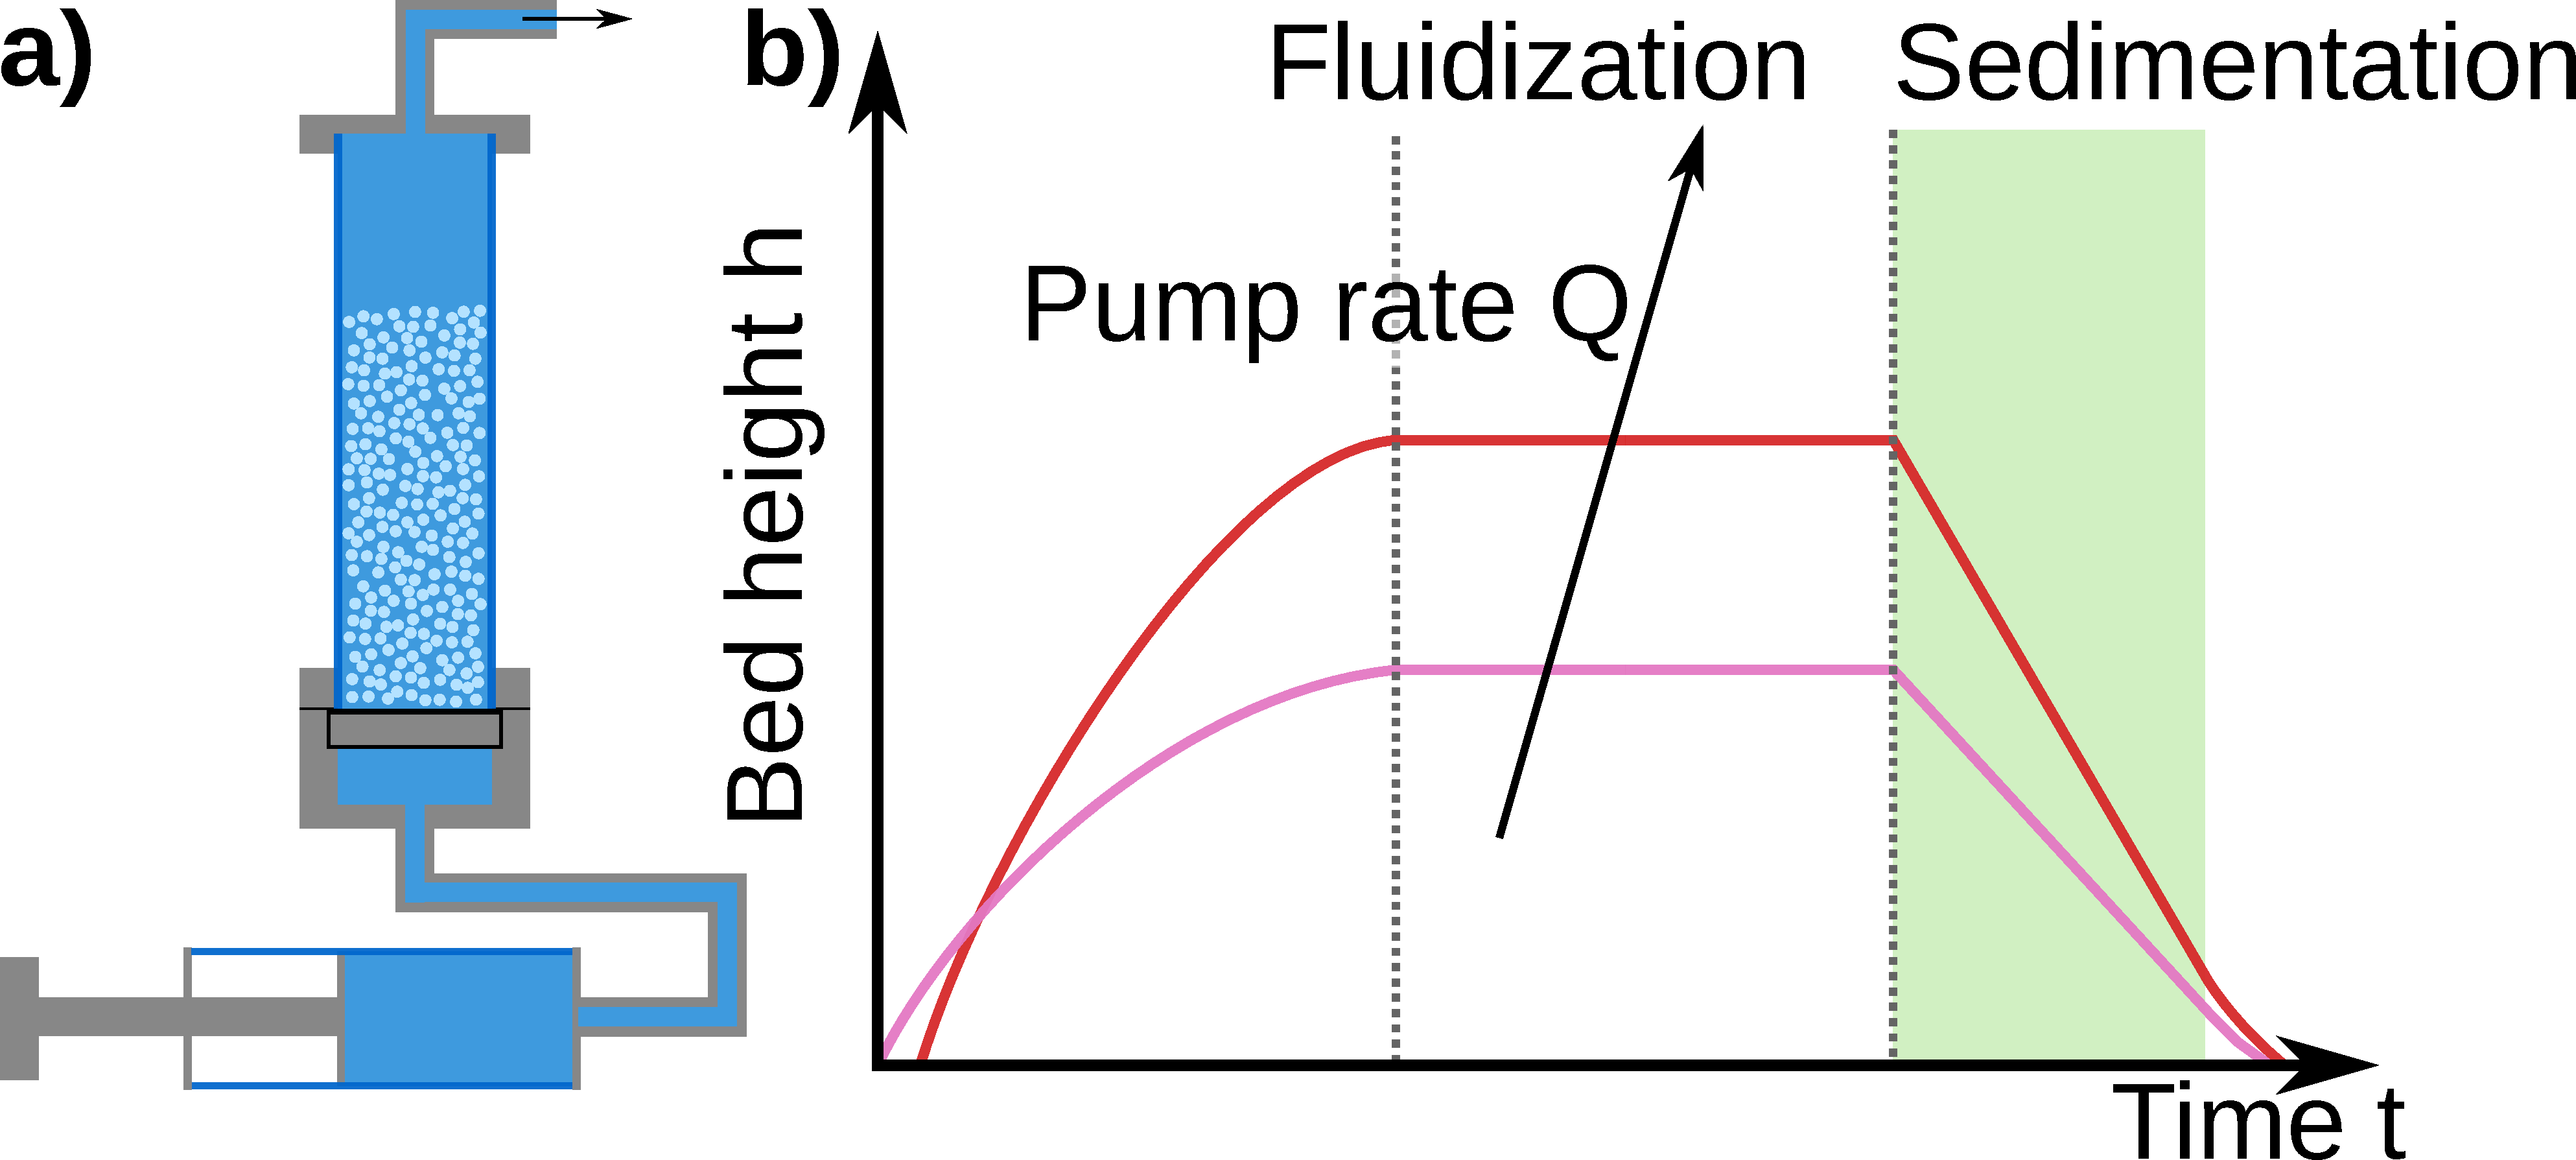
\includegraphics[width=0.8\textwidth]
{Sources/sedimenting_bed/setup-fluidized_bed_animation_2.pdf}}
\visible<3->{
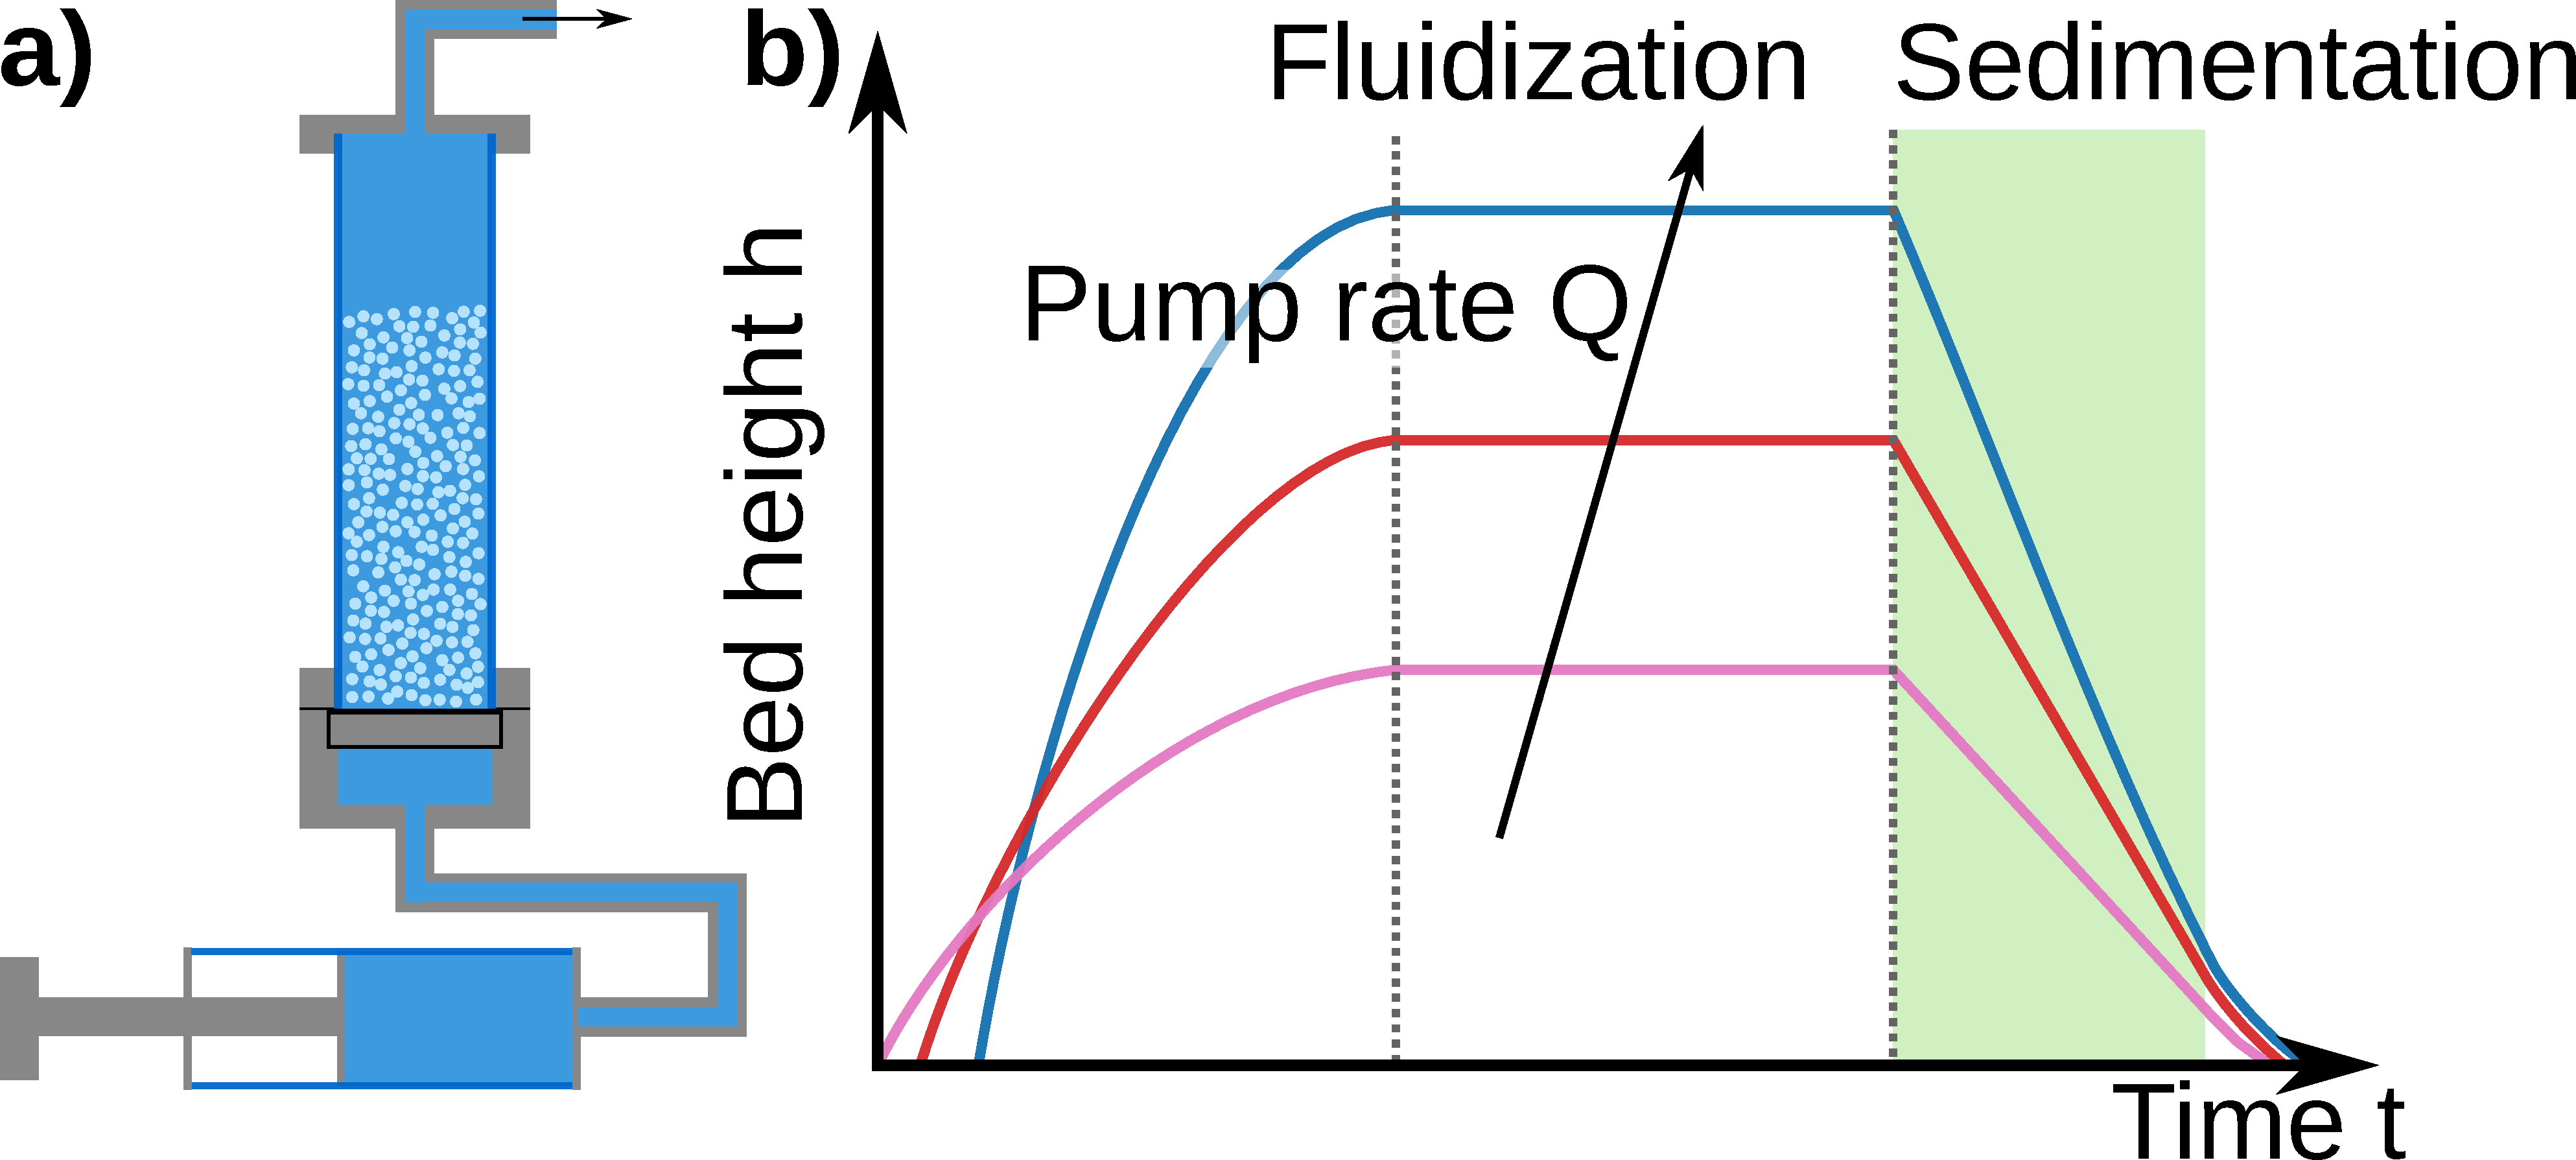
\includegraphics[width=0.8\textwidth]
{Sources/sedimenting_bed/setup-fluidized_bed_animation.pdf}}
\end{textblock}

\begin{textblock}{0.5}(0.5,0.4)
\centering
\visible<5->{
\movie[width =0.8\textwidth, poster, loop]	
{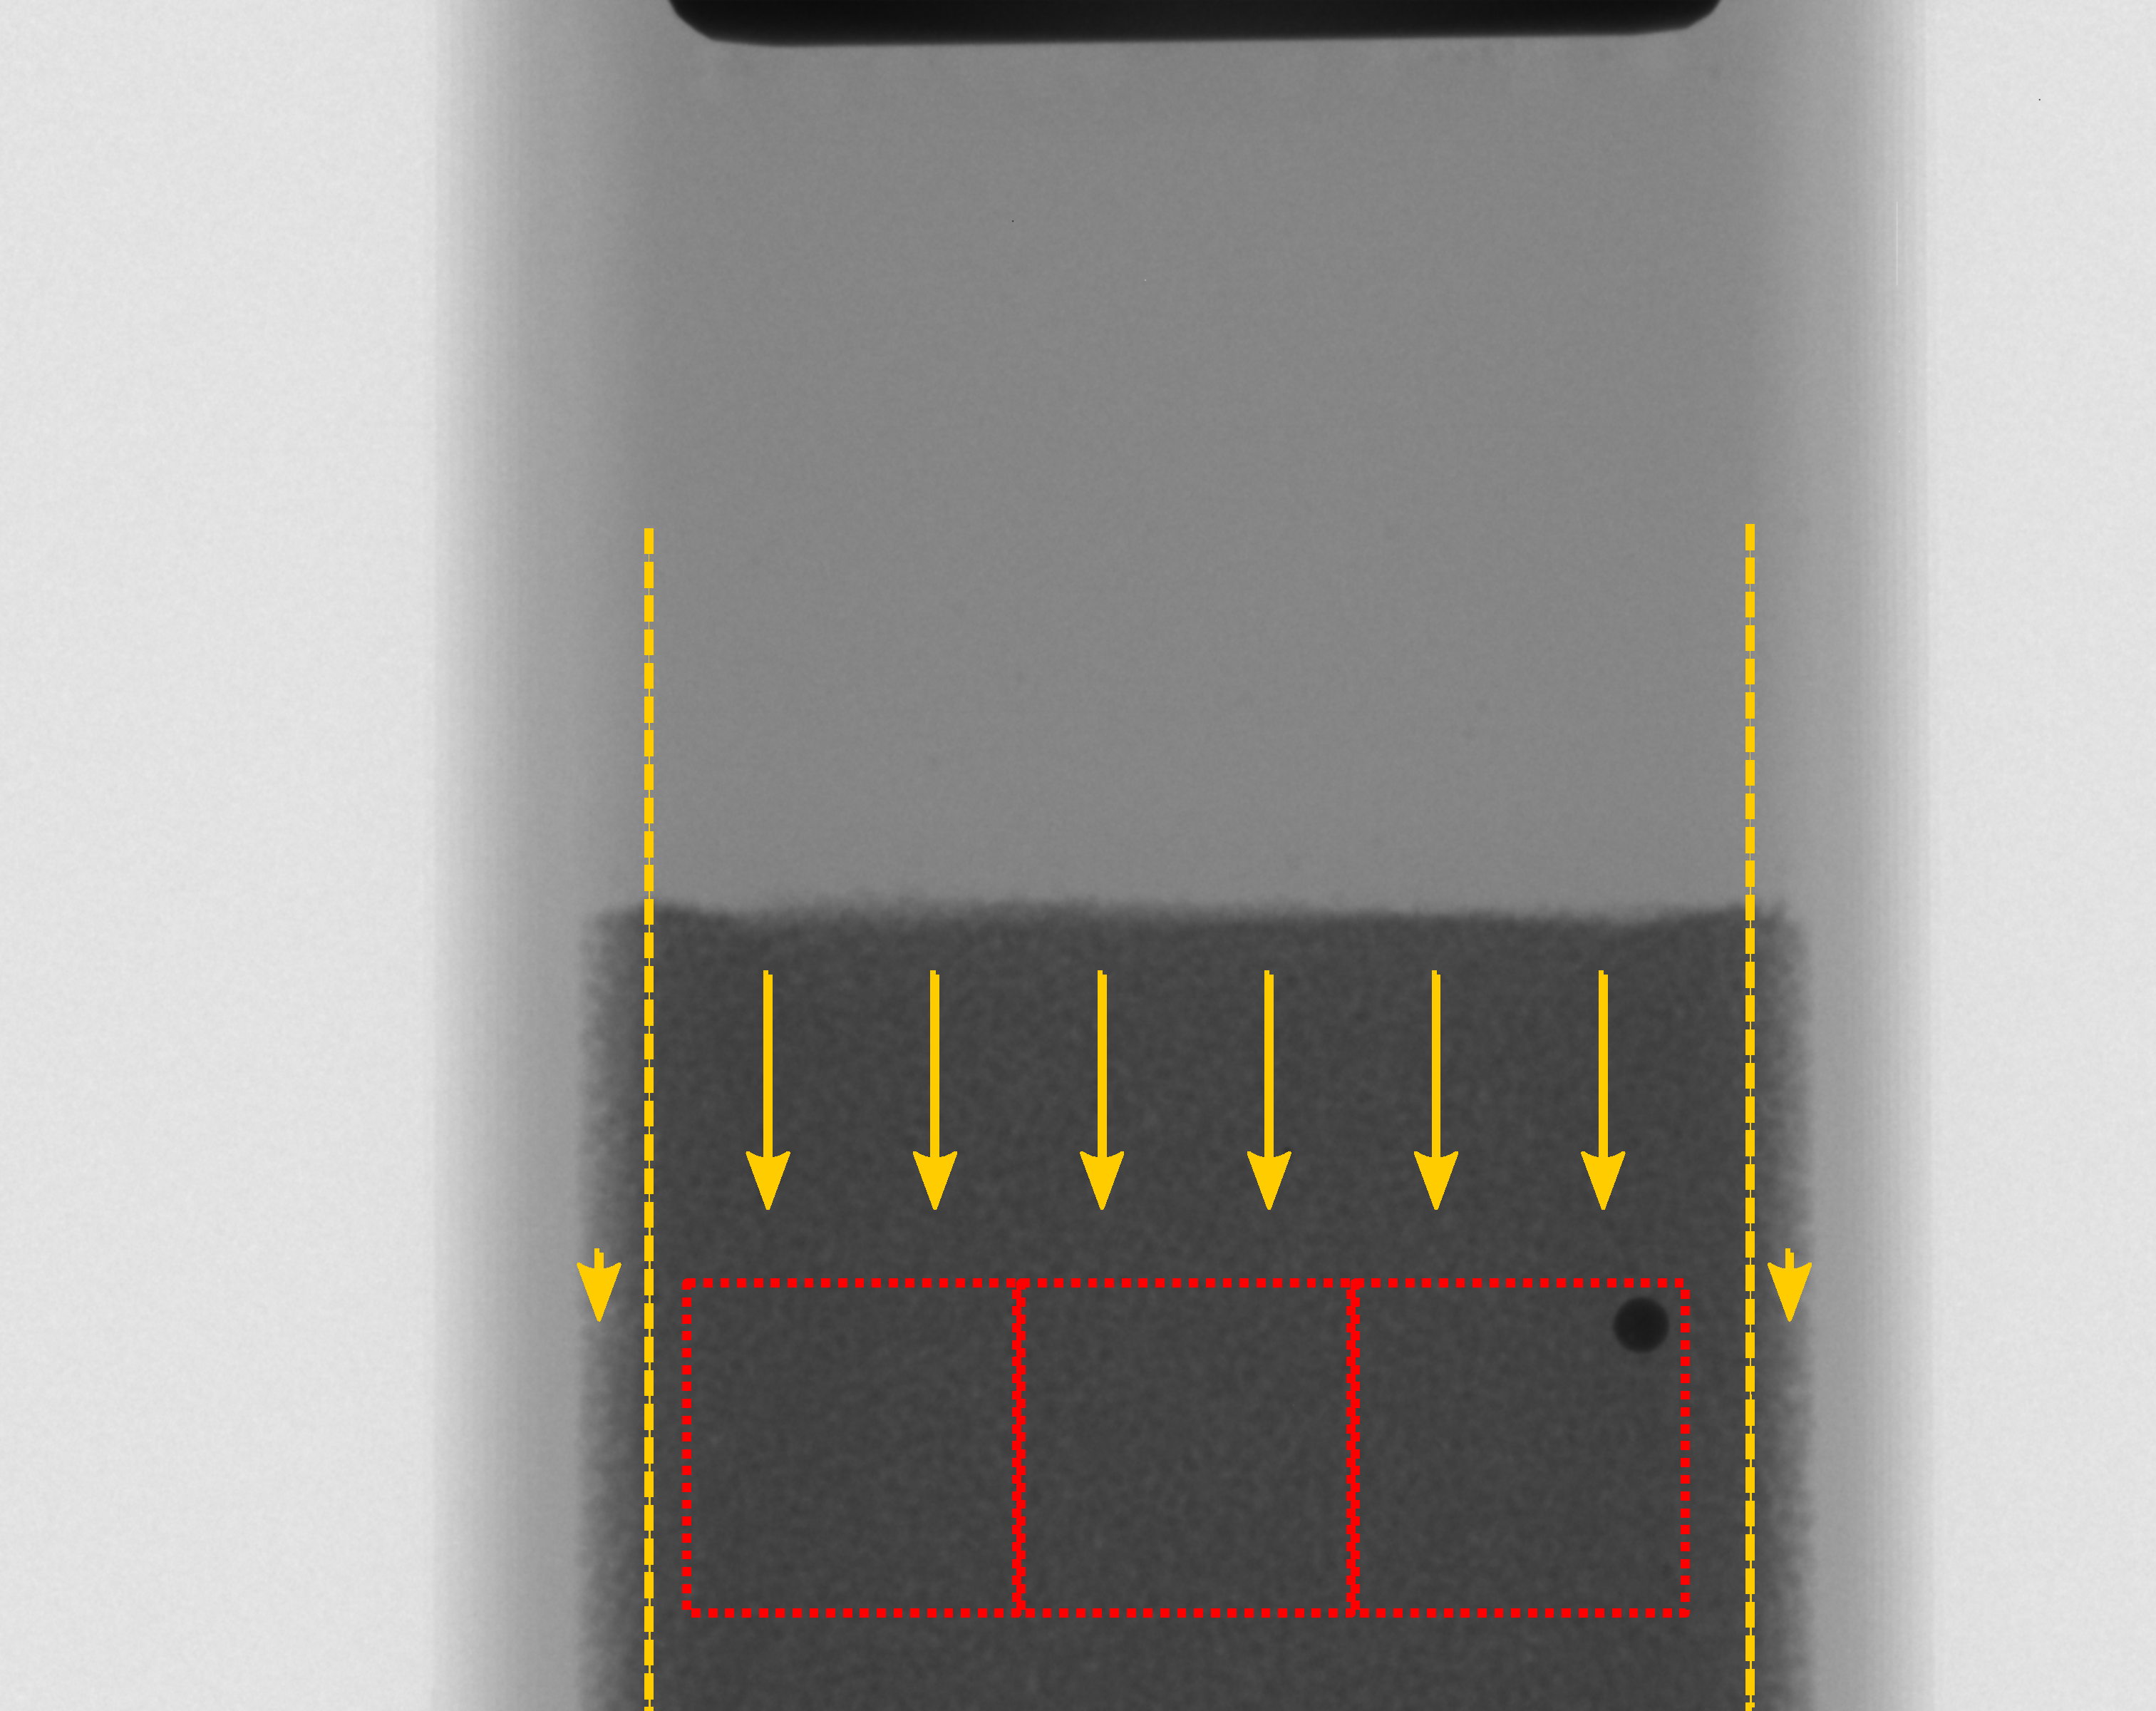
\includegraphics[width=0.8\textwidth]
{Sources/sedimenting_bed/creeping_boundary_flow.pdf}}
{videos/boundary_layer.avi}}
\end{textblock}

\begin{textblock}{0.45}(0.02,0.9)
\centering
\visible<4->{
$\langle v\rangle_\text{xdfa} > \langle v \rangle_\text{front}$ by 9.4\%}
\end{textblock}
}


%%%%%%%%%% Conclusion
\frame{
\begin{tikzpicture}[remember picture,overlay]
\fill[blue1]
(current page.north west) rectangle ([xshift=0.2\paperwidth,yshift=0.33\paperheight]current page.west|-{pic cs:end});
\end{tikzpicture}

\begin{textblock}{0.8}(0.02,0.03)
	\textcolor{white}{
		\Large Conclusion}
\end{textblock}

\begin{textblock}{0.46}(0.02,0.13)
\visible<1->{
\centering
\textbf{\Large Correction of beam hardening}
\vspace{-0.3cm}
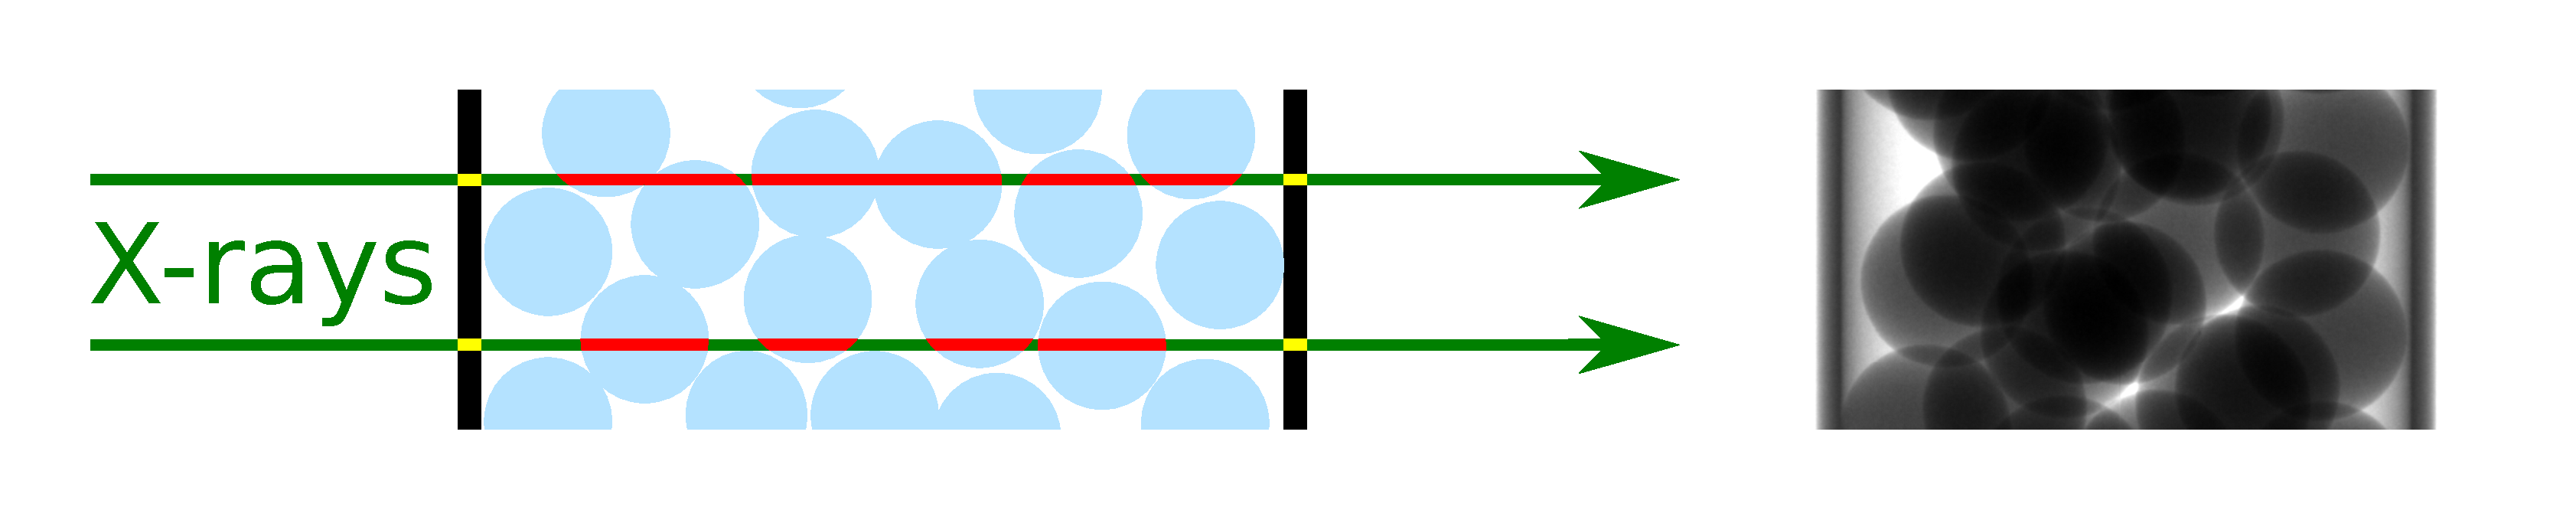
\includegraphics[width=0.9\textwidth]
{Sources/beam_hardening/2beams_attenuation_marked.pdf}

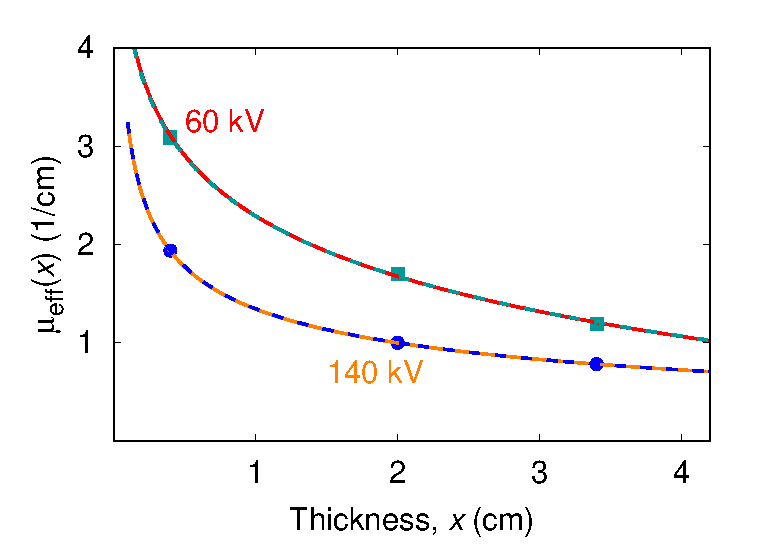
\includegraphics[width=\textwidth]
{Sources/beam_hardening/3datapoints_conclusion.eps}
}
\end{textblock}

\begin{textblock}{0.1}(0.2,0.45)
\visible<1->{
\colorbox{blue1}{\textcolor{white}{
$\boldsymbol{\mu_\text{eff}(x) = a + \frac{b}{x^\alpha}}$
}}}
\end{textblock}

\begin{textblock}{0.46}(0.5,0.13)
\visible<2->{
\centering
\textbf{\Large X-ray Digital Fourier Analysis}

\begin{minipage}[c]{0.6\textwidth}
\textbf{Synthetic radiograms}\\
\xcancel{Particle Tracking}\\
\xcancel{PIV}
\end{minipage}
\hfill
\begin{minipage}[c]{0.33\textwidth}
\fbox{\parbox{\textwidth}{
	\movie[width = \textwidth]
	{
\includegraphics[width=\textwidth]{Sources/X-DFA/100000_particles_fake_img.png}}
	{videos/100000_particles.avi}}}
\end{minipage}
\vspace{0.2cm}
\vfill

\begin{minipage}[c]{0.6\textwidth}
\textbf{Experimental validation}\\[0.1cm]
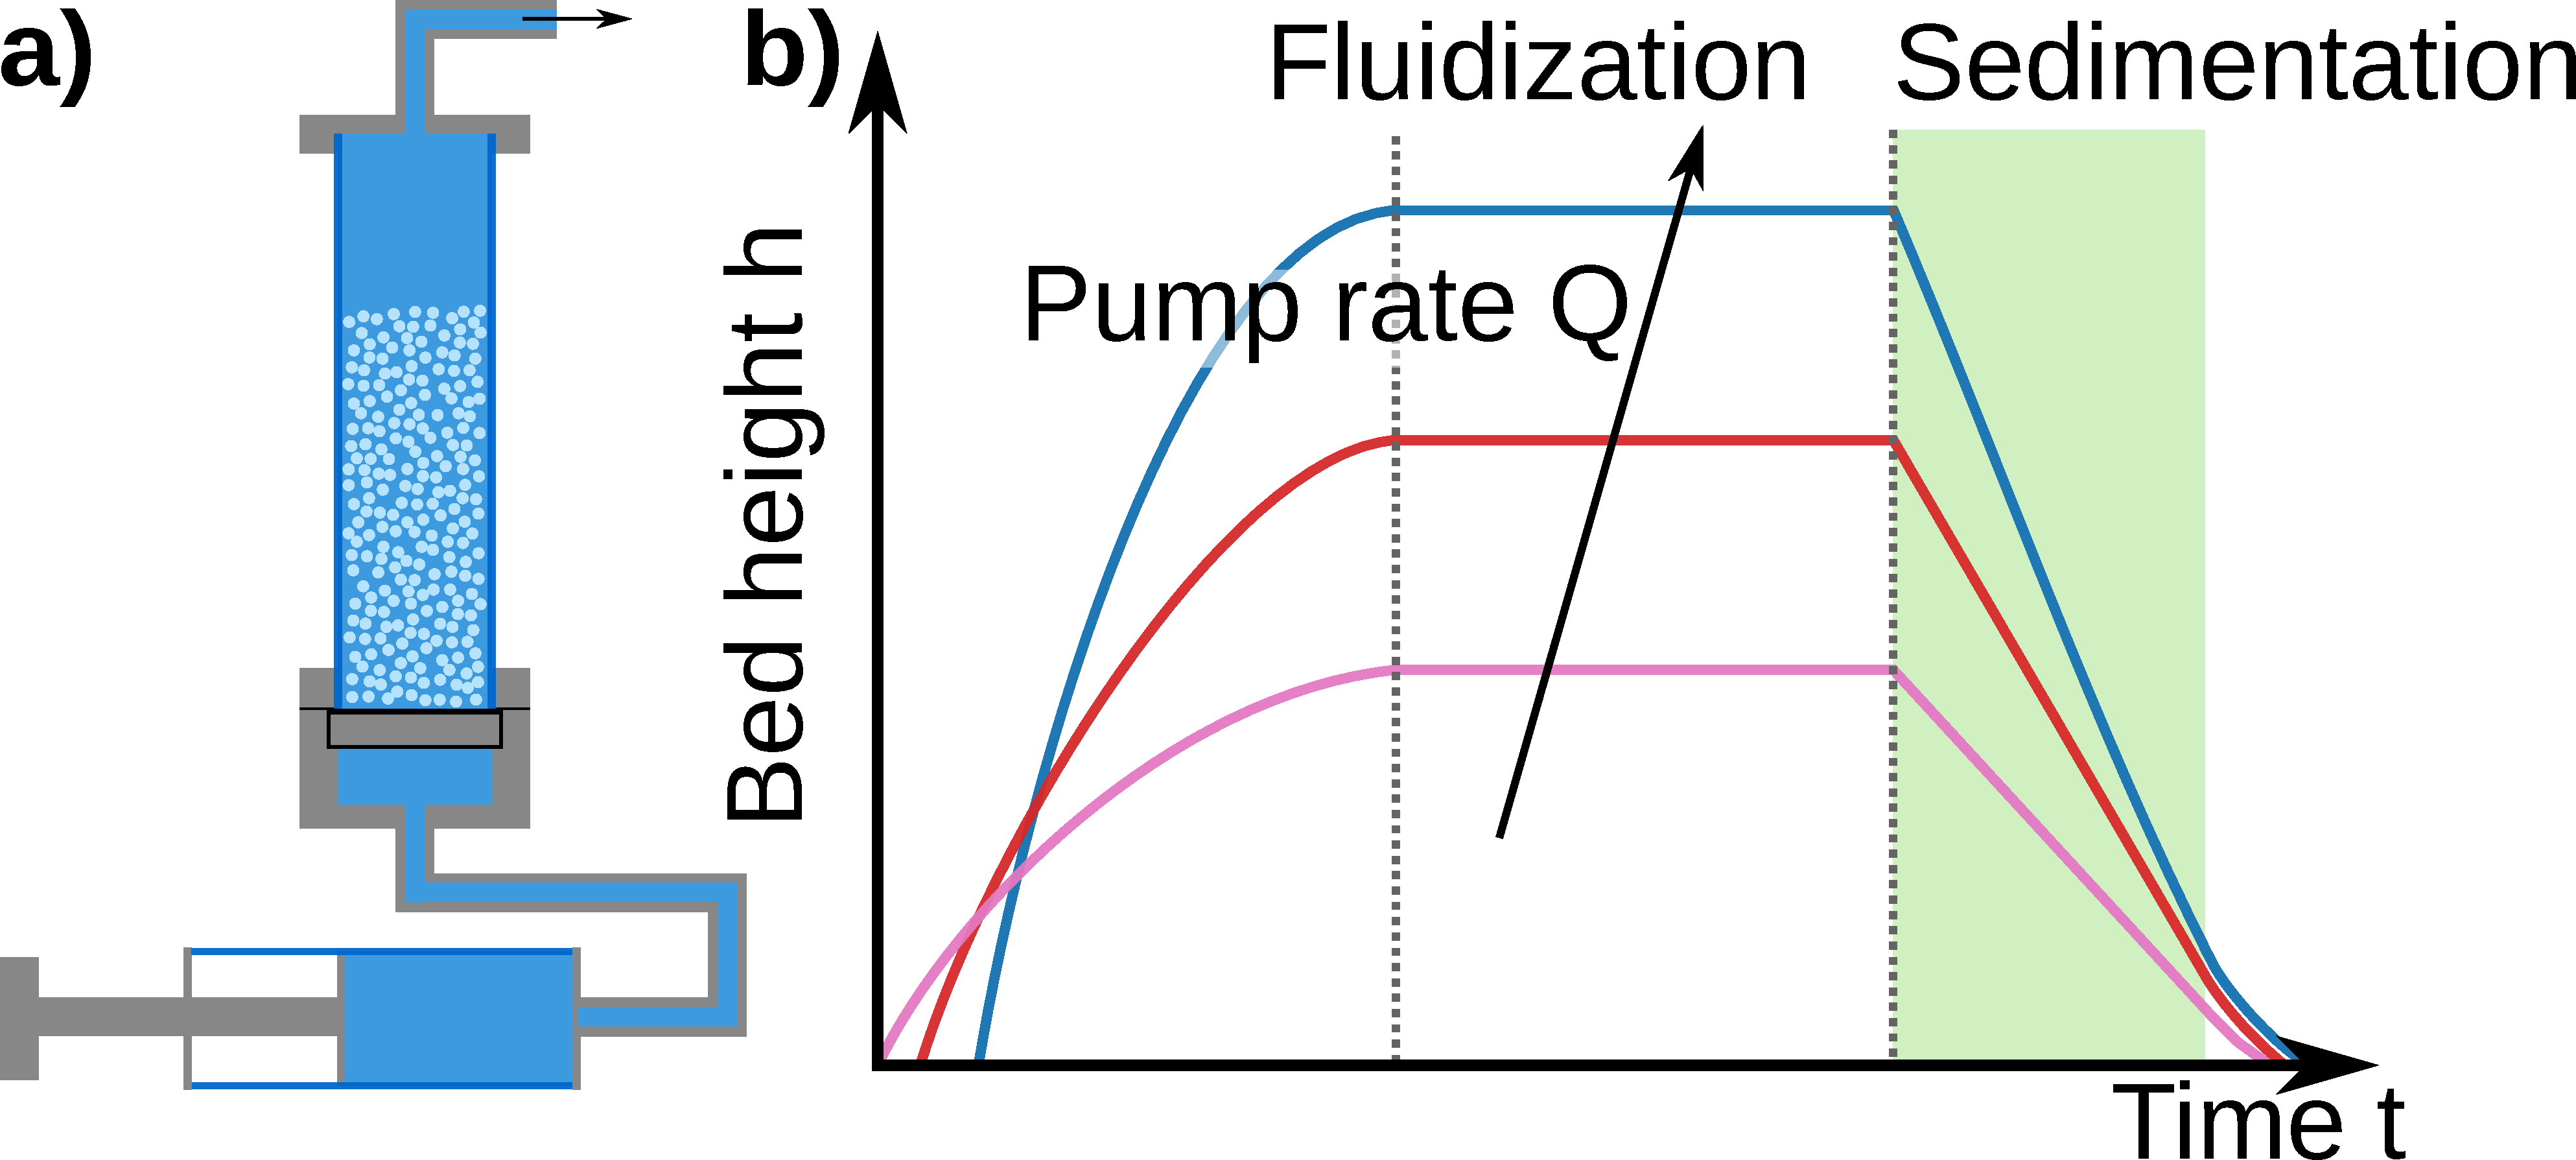
\includegraphics[width=\textwidth]
{Sources/sedimenting_bed/setup-fluidized_bed_animation.pdf}
\end{minipage}
\hfill
\begin{minipage}[c]{0.33\textwidth}
\fbox{\parbox{\textwidth}{
	\movie[width =\textwidth]
	{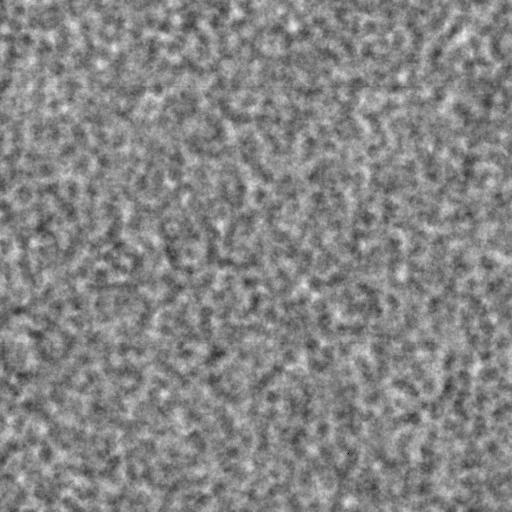
\includegraphics[width=\textwidth]{Sources/sedimenting_bed/sedimentationROI.png}}
	{videos/02_750ul_per_min_original.avi}}}
\end{minipage}
}
\end{textblock}


\begin{textblock}{0.4}(0.3,0.9)
\visible<3->{
\colorbox{lightred}{Temporal resolution of X-ray radiography}
}
\end{textblock}

}



%%%%%%%%% Thanks
\frame{
\begin{textblock}{1.}(0.0,0.0)
	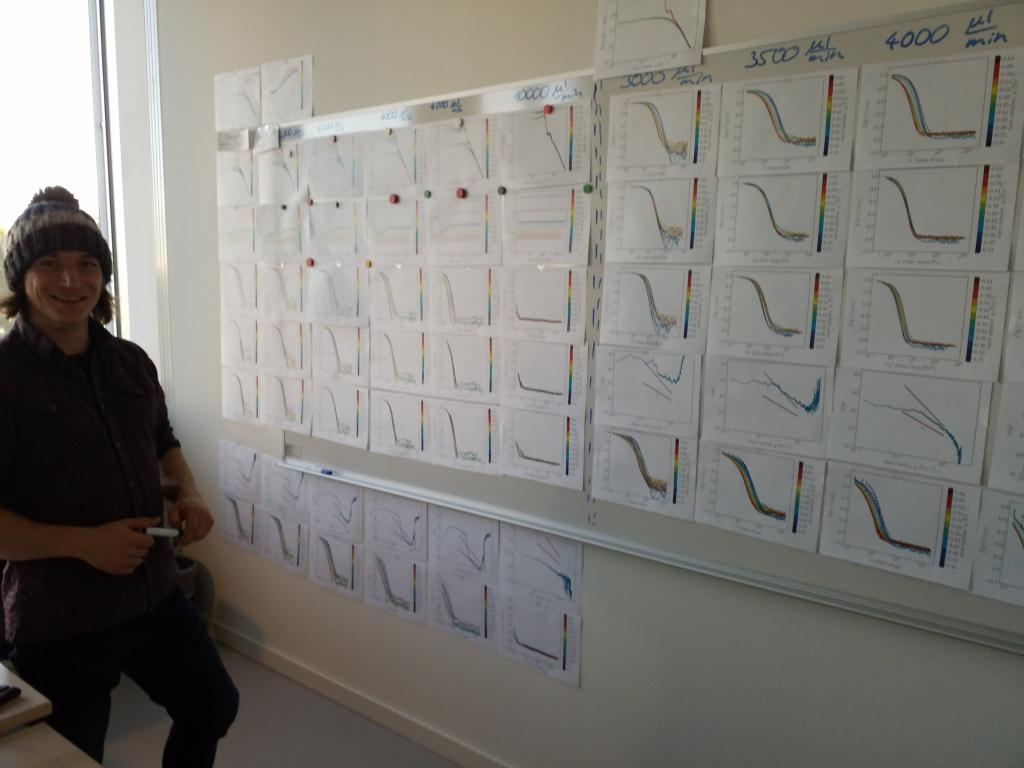
\includegraphics[width=\textwidth]
	{Sources/sedimenting_bed/whiteboard.jpg}
\end{textblock}

\begin{textblock}{0.8}(0.2,0.3)
	\colorbox{blue1}{\Huge \textcolor{white}{Thank you for your attention!}}
\end{textblock}
}



